%!TEX root = ../larxxia.tex

\section{Measure changes to matrices}
\label{sec:mctm}
\secttoc




\subsection{Compress images optimally}
\label{sec:ciio}

\index{image compression|(}

Photographs and other images take a lot of storage.
Reducing the amount of storage for an image, both for storage and for transmission, is essential.
The well-known \idx{jpeg} format for compressing photographs is incredibly useful: the \svd\ provides a related effective method of compression.

\begin{comment} 
Introduce digital {image compression} by \svd{}s \pooliv{p.607--8} \holti{p.336--7}  \cite[\S07]{Davis99a}  \cite[Ch.~9, 11]{Chartier2015}
\end{comment}


These \svd\ methods find approximate matrices of the images with the matrices having of various ranks.
Recall that a matrix of rank~\(k\) (Definition~\ref{def:rank}) means the matrix has precisely \(k\)~non-zero singular values, that is, an \(m\times n\) matrix
\begin{eqnarray*}
A&=&\usv
\\&=&
\begin{bmatrix} \uv_1&\cdots&\uv_k&\cdots&\uv_m \end{bmatrix}
\begin{bmatrix} \begin{matrix} \sigma_1&\cdots&0\\
\vdots&\ddots&\vdots\\
0&\cdots&\sigma_k \end{matrix} & 
O_{k\times (n-k)}\\\,\\
O_{(m-k)\times k}&O_{(m-k)\times (n-k)}\end{bmatrix}
\tr V
\\&&(\text{upon multiplying the form of the first two matrices})
\\&=&
\begin{bmatrix} \sigma_1\uv_1&\cdots&\sigma_k\uv_k&O_{m\times(n-k)} \end{bmatrix}
\begin{bmatrix} \tr\vv_1\\\vdots\\\tr\vv_k\\\vdots\\\tr\vv_n \end{bmatrix}
\\&&(\text{upon multiplying the form of these two matrices})
\\&=&
\sigma_1\uv_1\tr\vv_1+\sigma_2\uv_2\tr\vv_2+\cdots+\sigma_k\uv_k\tr\vv_k\,.
\end{eqnarray*}
This last form constructs matrix~\(A\).
Further, this last form \emph{has relatively few components when the rank~\(k\) is low} compared to~\(m\) and~\(n\).




\begin{example} \label{eg:}
Invent and write down a rank three representation of the \(5\times5\) `\idx{bulls eye}' matrix (illustrated in the margin)
\marginpar{\input{ApproxMat/bullseye.ltx}}
\begin{equation*}
A=\begin{bmatrix} 0&1&1&1&0
\\1&0&0&0&1
\\1&0&1&0&1
\\1&0&0&0&1
\\0&1&1&1&0 \end{bmatrix}.
\end{equation*}
\begin{solution} 
Here we set all coefficients \(\sigma_1=\sigma_2=\sigma_3=1\) and let the vectors set the magnitude (here these are not singular vectors and \(\sigma_j\)~are not singular values---but subsequently such a meaning will be restored).
\begin{enumerate}
\item Arbitrarily start by addressing together the first and last rows of the image (as illustrated): they are computed by choosing  \(\uv_1=(1,0,0,0,1)\) and \(\vv_1=(0,1,1,1,0)\), and using the rank one matrix
\marginpar{\input{ApproxMat/bulls1.ltx}}
\begin{equation*}
\uv_1\tr\vv_1
=\begin{bmatrix} 1\\0\\0\\0\\1 \end{bmatrix}
\begin{bmatrix} 0&1&1&1&0 \end{bmatrix}
=\begin{bmatrix} 0&1&1&1&0
\\0&0&0&0&0
\\0&0&0&0&0
\\0&0&0&0&0
\\0&1&1&1&0 \end{bmatrix}.
\end{equation*}

\item Next choose to address together the first and last columns of the image (as illustrated): they are computed by choosing  \(\uv_2=(0,1,1,1,0)\) and \(\vv_2=(1,0,0,0,1)\), and using the rank two matrix
\marginpar{\input{ApproxMat/bulls2.ltx}}
\begin{eqnarray*}
\uv_1\tr\vv_1+\uv_2\vv_2
&=&\uv_1\tr\vv_1+\begin{bmatrix} 0\\1\\1\\1\\0 \end{bmatrix}
\begin{bmatrix} 1&0&0&0&1 \end{bmatrix}
\\&=&\uv_1\tr\vv_1+\begin{bmatrix} 0&0&0&0&0
\\1&0&0&0&1
\\1&0&0&0&1
\\1&0&0&0&1
\\0&0&0&0&0 \end{bmatrix}
\\&=&\begin{bmatrix} 0&1&1&1&0
\\1&0&0&0&1
\\1&0&0&0&1
\\1&0&0&0&1
\\0&1&1&1&0 \end{bmatrix}.
\end{eqnarray*}

\item Lastly put the dot in the middle of the image (to form the original): choose  \(\uv_3=\vv_3=(0,0,1,0,0)\), and compute the rank three matrix
\begin{eqnarray*}
&&\uv_1\tr\vv_1+\uv_2\vv_2+\uv_3\vv_3
\\&=&\uv_1\tr\vv_1+\uv_2\vv_2
+\begin{bmatrix} 0\\0\\1\\0\\0 \end{bmatrix}
\begin{bmatrix} 0&0&1&0&0 \end{bmatrix}
\\&=&\uv_1\tr\vv_1+\uv_2\vv_2+\begin{bmatrix} 0&0&0&0&0
\\0&0&0&0&0
\\0&0&1&0&0
\\0&0&0&0&0
\\0&0&0&0&0 \end{bmatrix}
\\&=&\begin{bmatrix} 0&1&1&1&0
\\1&0&0&0&1
\\1&0&1&0&1
\\1&0&0&0&1
\\0&1&1&1&0 \end{bmatrix}.
\end{eqnarray*}

\end{enumerate}
\end{solution}
\end{example}




\begin{activity}
Which pair of vectors gives a rank one representation,~\(\uv\tr\vv\) of the matrix
\marginpar{\input{ApproxMat/actone.ltx}}%
\begin{equation*}
\begin{bmatrix} 0&1&1&0 
\\0&0&0&0
\\0&1&1&0
\\0&1&1&0 \end{bmatrix}?
\end{equation*}
\begin{enumerate}
\item \(\uv=(0,1,1,0)\), \(\vv=(1,0,1,1)\)
\item \(\uv=(0,1,1,0)\), \(\vv=(1,1,0,1)\)
\item \(\uv=(1,0,1,1)\), \(\vv=(0,1,1,0)\)\actans
\item \(\uv=(1,1,0,1)\), \(\vv=(0,1,1,0)\)
\end{enumerate}
\end{activity}





\begin{procedure}[approximate images] \label{pro:ai} 
For an image stored as scalars in an \(m\times n\) matrix~\(A\).
\begin{enumerate}
\item Compute an \svd\ \(A=\usv\) with \verb|[U,S,V]=svd(A)|.
\item Choose a desired \idx{rank}~\(k\) based upon the \idx{singular value}s (Theorem~\ref{thm:am}): typically there will be \(k\)~`large' \idx{singular value}s and the rest are `small'.
\item Then the `best' rank~\(k\) approximation to the image matrix~\(A\) is (using the subscript~\(k\) on the matrix name to denote the rank~\(k\) approximation)
\begin{eqnarray*}
A_k&:=&\sigma_1\uv_1\tr\vv_1+\sigma_2\uv_2\tr\vv_2+\cdots+\sigma_k\uv_k\tr\vv_k
\\&=&\verb|U(:,1:k)*S(1:k,1:k)*V(:,1:k)'|
\end{eqnarray*}
\end{enumerate}
\end{procedure}






\begin{example} \label{eg:bullseyemat}
Use Procedure~\ref{pro:ai} to find the `best' rank two matrix, and also the `best' rank three matrix, to approximate the `bulls eye' image matrix (illustrated in the margin)
\marginpar{\input{ApproxMat/bullseye.ltx}}
\begin{equation*}
A=\begin{bmatrix} 0&1&1&1&0
\\1&0&0&0&1
\\1&0&1&0&1
\\1&0&0&0&1
\\0&1&1&1&0 \end{bmatrix}.
\end{equation*}
\begin{solution} 
Enter the matrix into \script\ and compute an \svd, \(A=\usv\), with \verb|[U,S,V]=svd(A)| to find \twodp
\begin{verbatim}
U =
  -0.47   0.51   0.14   0.71   0.05
  -0.35  -0.44   0.43  -0.05   0.71
  -0.56  -0.31  -0.77   0.00   0.00
  -0.35  -0.44   0.43   0.05  -0.71
  -0.47   0.51   0.14  -0.71  -0.05
S =
   2.68      0      0      0      0
      0   2.32      0      0      0
      0      0   0.64      0      0
      0      0      0   0.00      0
      0      0      0      0   0.00
V =
  -0.47  -0.51   0.14  -0.68  -0.18
  -0.35   0.44   0.43  -0.18   0.68
  -0.56   0.31  -0.77   0.00  -0.00
  -0.35   0.44   0.43   0.18  -0.68
  -0.47  -0.51   0.14   0.68   0.18
\end{verbatim}
\setbox\ajrqrbox\hbox{\qrcode{% approx bulls eye image
A=[0 1 1 1 0
   1 0 0 0 1
   1 0 1 0 1
   1 0 0 0 1
   0 1 1 1 0]
[U,S,V]=svd(A)
A3=U(:,1:3)*S(1:3,1:3)*V(:,1:3)'
A2=U(:,1:2)*S(1:2,1:2)*V(:,1:2)'
}}%
\marginpar{\usebox{\ajrqrbox\\[2ex]}}%
\begin{itemize}
\item For this matrix there are three `large' singular values of~\(2.68\), \(2.32\) and~\(0.64\), and two `small' singular values of~\(0.00\) (they are precisely zero), thus construct a rank three approximation to the image matrix as
\begin{equation*}
A_3=\sigma_1\uv_1\tr\vv_1+\sigma_2\uv_2\tr\vv_2+\sigma_3\uv_3\tr\vv_3,
\end{equation*}
computed with \verb|A3=U(:,1:3)*S(1:3,1:3)*V(:,1:3)'|, giving \twodp
\begin{verbatim}
A3 =
   0.00   1.00   1.00   1.00   0.00
   1.00   0.00   0.00   0.00   1.00
   1.00   0.00   1.00   0.00   1.00
   1.00   0.00   0.00   0.00   1.00
  -0.00   1.00   1.00   1.00  -0.00
\end{verbatim}
The rank~3 matrix~\(A_3\) exactly reproduces the image matrix~\(A\). 
This exactness is due to the  fourth and fifth singular values being precisely zero (to numerical error).

\item Alternatively, in the context of some application, we could subjectively decide that there are two `large' singular values of~\(2.68\) and~\(2.32\), and three `small' singular values of~\(0.64\) and~\(0.00\).
In such a case, construct a rank two approximation to the image matrix as (illustrated in the margin)
\marginpar{\input{ApproxMat/bullseye2.ltx}}
\begin{equation*}
A_2=\sigma_1\uv_1\tr\vv_1+\sigma_2\uv_2\tr\vv_2,
\end{equation*}
computed with \verb|A2=U(:,1:2)*S(1:2,1:2)*V(:,1:2)'|, giving \twodp
\begin{verbatim}
A2 =
  -0.01   0.96   1.07   0.96  -0.01
   0.96  -0.12   0.21  -0.12   0.96
   1.07   0.21   0.62   0.21   1.07
   0.96  -0.12   0.21  -0.12   0.96
  -0.01   0.96   1.07   0.96  -0.01
\end{verbatim}
This rank two approximation~\(A_2\) is indeed roughly the same as the image matrix~\(A\), albeit with errors of~20\% or so.
Subsequent theory confirms that the relative error is characterised by \(\sigma_3/\sigma_1=0.24\) here.
\end{itemize}
\end{solution}
\end{example}




\begin{activity}
%r=2
%a=randn(4)
%[u,s,v]=svd(a);
%u=round(abs(u)*2)/2,v=round(abs(v)*2)/2
%A=u(:,1:r)*v(:,1:r)'
%[U,S,V]=svd(A)
A given image, shown in the margin, has matrix with \svd\ \twodp
\marginpar{\input{ApproxMat/acttwo.ltx}}%
\begin{verbatim}
U =
  -0.72   0.48   0.50  -0.00
  -0.22  -0.84   0.50  -0.00
  -0.47  -0.18  -0.50  -0.71
  -0.47  -0.18  -0.50   0.71
S =
   2.45      0      0      0
      0   0.37      0      0
      0      0   0.00      0
      0      0      0   0.00
V =
  -0.43  -0.07   0.87  -0.24
  -0.43  -0.07  -0.44  -0.78
  -0.48   0.83  -0.11   0.26
  -0.62  -0.55  -0.21   0.51
\end{verbatim}
What rank representation will exactly reproduce the matrix\slash image?
\partswidth=5em
\begin{parts}
\item 1
\item 2
\item 3
\item 4
\end{parts}
\end{activity}





\begin{example} \label{eg:euler1737}
In the margin is a \(326\times277\) greyscale image of \idx{Euler} at 30~years old.  
\marginpar{\raggedright
Euler, 1737, by Vasilij Sokolov
\includegraphics[width=\linewidth]{ApproxMat/euler1737} 
\url{http://eulerarchive.maa.org/portraits/portraits.html} [Sep 2015]}
As such the image is coded as \(90\,302\)~scalar numbers.
Let's find a good approximation to the image that uses much fewer numbers, and hence takes less storage.
That is, we will effectively compress the image.

\begin{solution} 
We use an \svd\ to approximate the image of Euler to controllable levels of approximation.
For example, Figure~\ref{fig:euler1737rank} shows four approximations to the image of Euler, ranging from the hopeless (labelled ``rank~3'')  to the original (labelled ``rank~277'').
\begin{figure}
\caption{four approximate images of Euler ranging from the poor rank~\(3\), via the adequate rank~\(10\), the good rank~\(30\), to the original rank~\(277\).}
\label{fig:euler1737rank}
\centering
\includegraphics{ApproxMat/euler1737rank}
\end{figure}

Procedure~\ref{pro:ai} is as follows.
\begin{itemize}
\item First download the image from the website, and then read the image into \script\ using 
\begin{verbatim}
rgb=imread('euler1737.png');
A=mean(rgb,3);
\end{verbatim}
The \verb|imread| command sets the \(326\times277\times3\) array~\verb|rgb| to the red-green-blue values of the image data. 
Then convert into a grayscale image matrix~\verb|A| by averaging the red-green-blue values via the function \verb|mean(rgb,3)| which computes the mean over the third dimension of the array (over the three colours).

\item Compute an \svd, \(A=\usv\), of the matrix~\verb|A| with the usual command \verb|[U,S,V]=svd(A)|.
Here orthogonal~\verb|U| is \(326\times326\), diagonal \(\verb|S|=\diag(41\,422, 8\,309,  \ldots,0.79,0)\) is \(326\times277\), and orthogonal~\verb|V| is \(277\times277\).
These matrices are far too big to record in this text.
\setbox\ajrqrbox\hbox{\qrcode{% approx Euler
rgb=imread('euler1737.png');
A=mean(rgb,3);
[U,S,V]=svd(A); 
colormap('gray')
k=10
imagesc(U(:,1:k)*S(1:k,1:k)*V(:,1:k)')
axis equal, axis off
}}%
\marginpar{\usebox{\ajrqrbox\\[2ex]}}%


\begin{figure}
\caption{singular values of the image of Euler, 1737.}
\label{fig:euler1737sing}
\centering
%\includegraphics[width=\linewidth]{ApproxMat/euler1737sing}
\input{ApproxMat/euler1737sing.ltx}
\end{figure}
\item Figure~\ref{fig:euler1737sing} plots the non-zero singular values from largest to smallest: they cover a range of five orders of magnitude (the vertical axis is logarithmic).
Choose some number~\(k\) of singular vectors to use: \(k\)~is the rank of the approximate images in Figure~\ref{fig:euler1737rank}.
The choice may be guided by the decrease of these singular values: as discussed later, for a say 1\%~error choose~\(k\) such that \(\sigma_k\approx 0.01\sigma_1\) which from the index~\(j\) axis of Figure~\ref{fig:euler1737sing} is around \(k\approx 25\)\,.

\item Construct the approximate rank~\(k\) image
\begin{eqnarray*}
A_k&=&\sigma_1\uv_1\tr\vv_1+\sigma_2\uv_2\tr\vv_2+\cdots+\sigma_k\uv_k\tr\vv_k
\\&=&\verb|U(:,1:k)*S(1:k,1:k)*V(:,1:k)'|
\end{eqnarray*}

\item Let's say the rank~\(30\) image of Figure~\ref{fig:euler1737rank} is the desired good approximation.  
To reconstruct it we need \(30\)~singular values \hlist\sigma{30}, \(30\)~columns \hlist\uv{30}\ of~\(U\), \(30\)~columns \hlist\vv{30}\ of~\(V\) making a total of
\begin{equation*}
30+30\times326+30\times277=18\,120\text{ numbers}.
\end{equation*}
These \(18\,120\)~numbers are much fewer than (one fifth of) the \(326\times277=90,302\)~numbers of the original image.
The \svd\ provides an effective flexible data compression.
\end{itemize}
\end{solution}
\end{example}









\begin{table}
\caption{As well as the \script\ commands and operations listed in Tables~\ref{tbl:mtlbpre}, \ref{tbl:mtlbbasics}, \ref{tbl:mtlbops}, \ref{tbl:mtlbmops}, \ref{tbl:mtlbsvd}, and~\ref{tbl:mtlbimag}  we may invoke these functions.\index{Matlab@\textsc{Matlab}|textbf}\index{Octave|textbf}} \label{tbl:mtlbnorm}
\hrule
\begin{minipage}{\linewidth}
\begin{itemize}
\item \index{norm()@\texttt{norm()}}\verb|norm(A)| computes the \idx{matrix norm} of Definition~\ref{def:norm}, namely the largest \idx{singular value} of the matrix~\(A\).

Also, and consistent with the matrix norm, recall that \verb|norm(v)| for a vector~\verb|v| computes the \idx{length} \(\sqrt{v_1^2+v_2^2+\cdots+v_n^2}\).

%Whereas, \verb|norm(A,'fro')| computes the \idx{Frobenius norm}~\(\norm A_F\) defined such that \(\norm A_F^2=\sum_{i,j}a_{ij}^2\).

%\item \index{reshape()@\texttt{reshape()}}\verb|reshape(A,p,q)| for a \(m\times n\) matrix\slash vector~\(A\), provided \(mn=pq\)\,, generates a \(p\times q\) matrix with entries taken column-wise from~\(A\).  
%Either \(p\) or~\(q\) can be~\verb|[]| in which case \script\ uses \(p=mn/q\) or \(q=mn/p\) respectively.

\item \index{scatter()@\texttt{scatter()}}\verb|scatter(x,y,[],c)| draws a 2D scatter plot of points with coordinates in vectors~\verb|x| and~\verb|y|, each point with a colour determined by the corresponding entry of vector~\verb|c|.  

Similarly for \index{scatter3()@\texttt{scatter3()}}\verb|scatter3(x,y,z,[],c)| but in 3D.

\item \index{svds()@\texttt{svds()}}\verb|[U,S,V]=svds(A,k)| computes the \(k\)~largest singular values of the matrix~\(A\) in the diagonal of \(k\times k\) matrix~\(S\), and the  \(k\)~columns of~\(U\) and~\(V\) are the corresponding singular vectors.

%Whereas \verb|[U,S,V]=svds(A,k,s)| (for \(s\geq0\)) computes the \(k\)~singular values closest to~\(s\), and the corresponding singular vectors.

\item  \index{imread()@\texttt{imread()}}\verb|imread('|filename\verb|')| typically reads an image from a file into an \(m\times n\times 3\) array of red-green-blue values. 
The values are all `integers' in the range~\([0,255]\).

\item \index{mean()@\texttt{mean()}}\verb|mean(A)| of an \(m\times n\) array computes the \(n\)~elements in the row vector of \idx{average}s (the arithmetic mean) over each column of~\(A\).

Whereas \verb|mean(A,p)| for an \(\ell\)-dimensional array~\(A\) of dimension \(m_1\times m_2\times\cdots\times m_\ell\),  computes the mean over the \verb|p|th~index to give an array of size \(m_1\times\cdots\times m_{p-1}\times m_{p+1}\times\cdots\times m_\ell\).

\item \index{std()@\texttt{std()}}\verb|std(A)| of an \(m\times n\) array computes the \(n\)~elements in the row vector of the \idx{standard deviation} over each column of~\(A\) (close to the root-mean-square from the mean).

\item  \index{csvread()@\texttt{csvread()}}\verb|csvread('|filename\verb|')| reads data from a file into a matrix.
When each of the \(m\)~lines in the file is \(n\)~numbers separated by commas, then the result is an \(m\times n\) matrix. 

%\item \index{double@\texttt{double}}\verb|double(a)| converts the integers (or other data-types) in array~\verb|a| into the same size array of integer-valued real numbers that we normally use.
%\footnote{The term \emph{double} refers to the 15-digit precision of real numbers we use by default, compared to the \emph{single} precision of 7-digit real numbers used for simple purposes in, for example, graphics video cards for computers.}

\item \index{semilogy()@\texttt{semilogy()}}\verb|semilogy(x,y,'o')| draws a point plot of~\(y\) versus~\(x\) with the vertical axis being logarithmic.

%\item \index{figure@\texttt{figure}}\verb|figure(n)| starts or restarts drawing graphics into the figure window number~\verb|n|. 

%\item \index{colormap()@\texttt{colormap()}}\verb|colormap('gray')| \script\ usually draws graphs with colour, but for many images we need grayscale; this command changes the current figure to 64~shades of gray.  

%\item \index{subplot@\texttt{subplot}}\verb|subplot(m,n,p)| notionally tiles the current figure window into  \(\verb|m|\times\verb|n|\)~rectangular tiles, and then subsequent plotting commands draw into the \verb|p|th~tile numbered row-wise.
%For example, after \verb|subplot(2,3,p)| the~\verb|p| refers to the following tiles: \(\begin{array}{|c|c|c|} \hline 1&2&3\\ \hline 4&5&6\\ \hline \end{array}\).

%\item \index{imagesc()@\texttt{imagesc()}}\verb|imagesc(A)| where \(A\)~is a \(m\times n\) matrix of values draws an \(m\times n\) image in the current figure window using the values of~\(A\) (scaled to fit) to determine the colour from the current colormap (e.g., grayscale).

\item \index{axis@\texttt{axis}}\verb|axis| sets some properties of a drawn figure:
\begin{itemize}
\item \verb|axis equal| ensures horizontal and vertical directions are scaled the same---so here there is no distortion of the image;
\item \verb|axis off| means that the horizontal and vertical axes are not drawn---so here the image is unadorned.
\end{itemize}


\end{itemize}
\end{minipage}
\hrule
\end{table}








\subsection{Relate matrix changes to the SVD}
\label{sec:rmmsvd}


We need to define what `best' means in the approximation Procedure~\ref{pro:ai} and then show the procedure achieves this best.
%Recall diagonal matrices, orthogonal matrices and properties, rank, \svd\ factorisation, and how to approximate \idx{inconsistent} right-hand side vectors.
To proceed to understand \idx{image compression}, we need a measure of the magnitude of matrices and distances between matrices.

In linear algebra we use the double vertical bars,~\(\norm{\cdot}\), to  denote the magnitude of a matrix in order to avoid a notational clash with the well-established use of~\(|\cdot|\) for the determinant of a matrix (Chapter~\ref{ch:ddm}).

\begin{definition} \label{def:norm} 
Let \(A\) be an \(m\times n\) matrix.  
Define the \bfidx{matrix norm} (sometimes called the \idx{spectral norm})
\begin{equation}
\norm A:=\max_{|\xv|=1}|A\xv|, 
\quad\text{equivalently }\norm A=\sigma_1
\label{eq:}
\end{equation}
the largest \idx{singular value} of the matrix~\(A\).
\footnote{Sometimes this matrix norm is more specifically called a \idx{2-norm} and correspondingly denoted by~\(\norm{A}_2\): but not in this book because at other times and places \(\norm{A}_2\)~denotes something slightly different.}
\end{definition}
%\begin{proof} 
The equivalence, that \(\max_{|\xv|=1}|A\xv|=\sigma_1\)\,, is due to the definition of the largest singular value in the proof of the existence of an \svd\ (section~\ref{sec:psvdt}).
%\end{proof}



\begin{example} \label{eg:}
The two following \(2\times2\) matrices have the product~\(A\xv\) plotted~(red), adjoined to~\xv~(blue), for a complete range of unit vectors~\xv\ (as in section~\ref{sec:iee} for eigenvectors).
From Definition~\ref{def:norm}, the norm of the matrix~\(A\) is then the length of the longest such plotted~\(A\xv\).
\begin{aside}
The \script[1]\ function \index{eigshow()@\texttt{eigshow()}}\texttt{eigshow(A)} provides an interactive alternative to such static views.
\end{aside}%
For each matrix, use the plot to roughly estimate their norm.
\begin{enumerate}
\item\label{eg:g2x2norm:a} \(\eAii=\begin{bmatrix} 0.5&0.5\\-0.6&1.2 \end{bmatrix}\)\\
\marginpar{\eRose{0.5}{0.5}{-0.6}{1.2}}
\begin{solution} 
The longest \(\eAii\xv\) appear to be near the top and bottom of the plot, and appear to be a little longer than one, so estimate \(\norm{\eAii}\approx 1.3\)\,.
\end{solution}

\item \(\eAii=\begin{bmatrix} {-0.7}&{0.4}\\{0.6}&{0.5} \end{bmatrix}\)\\
\marginpar{\eRose{-0.7}{0.4}{0.6}{0.5}}
\begin{solution} 
Near the top and bottom of the plot, \(\eAii\xv\)~appears to be of length~\(0.6\).   
But the vectors pointing inwards from the right and left appear  longer at about~\(0.9\). 
So estimate \(\norm{\eAii}\approx 0.9\)\,.
\end{solution}

\end{enumerate}
\end{example}




\begin{example} \label{eg:}
Consider the \(2\times2\) matrix \(A=\begin{bmatrix} 1&1\\0&1 \end{bmatrix}\).
Explore products \(A\xv\) for unit vectors~\xv, and then find the \idx{matrix norm}~\(\norm{A}\).
\begin{itemize}
\item The standard unit vector \(\ev_2=(0,1)\) has \(|\ev_2|=1\) and \(A\ev_2=(1,1)\) has length \(|A\ev_2|=\sqrt2\)\,.
Since the matrix norm is the maximum of all possible~\(|A\xv|\), so \(\norm{A}\geq|A\ev_2|=\sqrt2\approx 1.41\)\,.
\item Another unit vector is \(\xv=(\tfrac35,\tfrac45)\).
Here \(A\xv=(\tfrac75,\tfrac45)\) has length \(\sqrt{49+16}/5=\sqrt{65}/5\approx1.61\)\,.
Hence the matrix norm \(\norm{A}\geq|A\xv|\approx 1.61\)\,.
\item To systematically find the norm, recall all unit vectors in 2D are of the form \(\xv=(\cos t,\sin t)\)\,.
Then
\begin{eqnarray*}
|A\xv|^2&=&|(\cos t+\sin t,\sin t)|^2
\\&=&(\cos t+\sin t)^2+\sin^2 t
\\&=&\cos^2 t+2\cos t\,\sin t+\sin^2t+\sin^2 t
\\&=&\tfrac32+\sin 2t-\tfrac12\cos 2t\,.
\end{eqnarray*}
This length (squared) is maximised (and minimised) for some~\(t\) determined by calculus.
Differentiating with respect to~\(t\)  leads to
\begin{equation*}
\frac{d|A\xv|^2}{dt}=2\cos2t+\sin 2t \ =0\quad\text{for stationary points.}
\end{equation*}
Rearranging determines we require \(\tan 2t=-2\)\,.
\marginpar{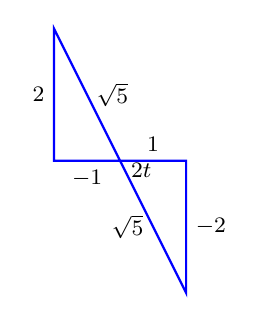
\begin{tikzpicture} 
\begin{axis}[small,font=\footnotesize
  ,axis equal image, axis lines=none, xmax=1.6, xmin=-1.4 ]  
  \addplot[blue,thick] coordinates {(0,0)(1,0)(1,-2)(-1,2)(-1,0)(0,0)};
  \node[] at (axis cs:0.32,-0.15) {$2t$};
  \node[right] at (axis cs:1,-1) {$-2$};
  \node[left] at (axis cs:-1,1) {$2$};
  \node[above] at (axis cs:0.5,0) {$1$};
  \node[below] at (axis cs:-0.5,0) {$-1$};
  \node[left] at (axis cs:0.5,-1) {$\sqrt5$};
  \node[right] at (axis cs:-0.5,1) {$\sqrt5$};
\end{axis}
\end{tikzpicture}}
The marginal right-angle triangles illustrate that a stationary point of~\(|A\xv|^2\) occurs for \(\sin 2t=\mp2/\sqrt5\) and correspondingly \(\cos2t=\pm1/\sqrt5\) (one gives a minimum and one gives the desired maximum).
Substituting these two cases gives
\begin{eqnarray*}
|A\xv|^2&=&\tfrac32+\sin 2t-\tfrac12\cos 2t
\\&=&\tfrac32\mp\tfrac2{\sqrt5}\mp\tfrac12\tfrac1{\sqrt5}
\\&=&\tfrac12(3\mp\sqrt5)
\\&=&\left(\frac{1\mp\sqrt5}2\right)^2.
\end{eqnarray*}
The plus alternative is the larger so gives the maximum, hence
\begin{equation*}
\norm{A}=\max_{|\xv|=1}|A\xv|=\frac{1+\sqrt5}2=1.6180\,.
\end{equation*}
\item Confirm with \script\ via \verb|svd([1 1;0 1])| which gives the singular values \(\sigma_1=1.6180\) and \(\sigma_2=0.6180\)\,.
Hence confirming the norm \(\norm{A}=\sigma_1=1.6180\)\,.

Alternatively, see Table~\ref{tbl:mtlbnorm}, execute \index{norm()@\texttt{norm()}}\verb|norm([1 1;0 1])| to compute the norm \(\norm{A}=1.6180\)\,.
\end{itemize}
\end{example}




\begin{activity}
%a=round(randn(3)*2)
%a=[1  -3  -2
%   1  -1   0
%   1   1  -2]
%[u,s,v]=svd(a)
A given \(3\times3\) matrix~\(A\) has the following products
\begin{equation*}
A\begin{bmatrix} 1\\0\\0 \end{bmatrix}
=\begin{bmatrix} 1\\1\\1 \end{bmatrix},\quad
A\begin{bmatrix} -1/3\\-2/3\\2/3 \end{bmatrix}
=\begin{bmatrix} 1/3\\1/3\\-7/3 \end{bmatrix},\quad
A\begin{bmatrix} 1\\-2\\-2 \end{bmatrix}
=\begin{bmatrix} 11\\3\\3 \end{bmatrix}.
\end{equation*}
Which of the following is the `best' statement about the norm of matrix~\(A\) (best in the sense of giving the largest valid lower bound)?
\begin{parts}
\item \(\|A\|\geq 1.7\)
\item \(\|A\|\geq 2.3\)
\item \(\|A\|\geq 3.9\)
\item \(\|A\|\geq 11.7\)
\end{parts}
\end{activity}




\begin{example} \label{eg:}
\script\ readily computes the \idx{matrix norm} either via an \svd\ or using the \verb|norm()| function directly (Table~\ref{tbl:mtlbnorm}).
Compute the norm of the following matrices.
\begin{enumerate}
\item \(A=\begin{bmatrix} 
   0.1&-1.3&-0.4&-0.1&-0.6\\
   1.9&2.4&-1.8&0.2&0.8\\
  -0.2&-0.5&-0.7&-2.5&1.1\\
  -1.8&0.2&1.1&-1.2&1.0\\
  -0.0&1.2&1.1&-0.1&1.7
 \end{bmatrix}\)
\begin{solution} 
Enter the matrix into \script\ then executing \verb|svd(A)| returns the vector of singular values
\setbox\ajrqrbox\hbox{\qrcode{% matrix norm
A=[0.1 -1.3 -0.4 -0.1 -0.6
   1.9 2.4 -1.8 0.2 0.8
  -0.2 -0.5 -0.7 -2.5 1.1
  -1.8 0.2 1.1 -1.2 1.0
  -0.0 1.2 1.1 -0.1 1.7]
svd(A)
norm(A)
}}%
\marginpar{\usebox{\ajrqrbox\\[2ex]}}%
\begin{equation*}
(4.0175,3.5044,2.6568,0.8571,0.1618),
\end{equation*}
so \(\norm{A}=\sigma_1=4.0175\)\,.
Alternatively, executing \index{norm()@\texttt{norm()}}\verb|norm(A)| directly gives  \(\norm{A}=4.0175\)\,.
\end{solution}

\item \(B=\begin{bmatrix} 
0&-2&-1&-4&-5&0
\\2&0&1&-2&-6&-2
\\-2&0&4&2&3&-3
\\1&2&-4&2&1&3
\end{bmatrix}\)
\begin{solution} 
Enter the matrix into \script\ then executing \verb|svd(B)| returns the vector of singular values
\setbox\ajrqrbox\hbox{\qrcode{% matrix norm
B=[0 -2 -1 -4 -5 0
 2 0 1 -2 -6 -2
 -2 0 4 2 3 -3
 1 2 -4 2 1 3]
svd(B)
norm(B)
}}%
\marginpar{\usebox{\ajrqrbox\\[2ex]}}%
\begin{equation*}
(10.1086,7.6641,3.2219,0.8352),
\end{equation*}
so \(\norm{B}=\sigma_1=10.1086\)\,.
Alternatively, executing \index{norm()@\texttt{norm()}}\verb|norm(B)| directly gives  \(\norm{B}=10.1086\)\,.
\end{solution}

\end{enumerate}
\end{example}










The Definition~\ref{def:norm} of the magnitude\slash norm of a matrix may appear a little strange, but, in addition to some marvellously useful properties, it nonetheless has all the familiar properties of a magnitude\slash length.
Recall from Chapter~\ref{ch:v} that for vectors:
\begin{itemize}
\item \(|\vv|=0\) if and only if \(\vv=\ov\) (Theorem~\ref{thm:veclen0});
\item \(|\uv\pm\vv|\leq|\uv|+|\vv|\) (the \idx{triangle inequality} of Theorem~\ref{thm:triscal});
\item \(|t\vv|=|t|\cdot|\vv|\) (Theorem~\ref{thm:triscal}).
\end{itemize}
Analogous properties hold for the matrix norm as established in the next theorem.




\begin{theorem}[norm properties] \label{thm:norm} 
Let \(A\) be an \(m\times n\) real matrix:
\begin{enumerate}
\item\label{thm:norm:iii} \(\norm A=0\) if and only if \(A=O_{m\times n}\)\,;
\item\label{thm:norm:vi} \(\norm{I_n}=1\)\,;
\item\label{thm:norm:iv} \(\norm {A\pm B}\leq\norm{A}+\norm B\), for every \(m\times n\) matrix~\(B\), is like a \idx{triangle inequality} (Theorem~\ref{thm:triscalc});
\item\label{thm:norm:v} \(\norm{tA}=|t|\norm{A}\)\,;
\item\label{thm:norm:i} \(\norm A=\norm{\tr A}\)\,;
\item\label{thm:norm:ii} \(\norm{Q_mA}=\norm A=\norm{AQ_n}\) for every \(m\times m\) \idx{orthogonal matrix}~\(Q_m\) and every \(n\times n\) \idx{orthogonal matrix}~\(Q_n\);
\item\label{thm:norm:viii} \(|A\xv|\leq\norm{A}|\xv|\) for all \(\xv\in\RR^n\), is like a \idx{Cauchy--Schwarz inequality} (Theorem~\ref{thm:triscalb}), as is the following;
\item\label{thm:norm:vii} \(\norm{AB}\leq\norm A\norm B\) for every \(n\times p\) matrix~\(B\).
\end{enumerate}
\end{theorem}
\begin{proof}  Alternative proofs to the following may be invoked (Exercise~\ref{ex:norm}).
Where necessary in the following, let matrix~\(A\) have the \svd\ \(A=\usv\).
\begin{itemize}
\item[\ref{thm:norm:iii}.]
If \(A=O_{m\times n}\) \,,
then from Definition~\ref{def:norm} 
\begin{equation*}
\norm A=\max_{|\xv|=1}|O\xv|
=\max_{|\xv|=1}|\ov|=\max_{|\xv|=1}0=0\,.
\end{equation*}
Conversely, if \(\norm A=0\)\,, then the largest singular value \(\sigma_1=0\) (Definition~\ref{def:norm}), which implies that all singular values are zero, so the matrix~\(A\) has an \svd\ of the form \(A=UO_{m\times n}\tr V\)\,, which evaluates to \(A=O_{m\times n}\)\,.

\item[\ref{thm:norm:vi}.] From Definition~\ref{def:norm}, 
\begin{equation*}
\norm{I_n}=\max_{|\xv|=1}|I_n\xv|
=\max_{|\xv|=1}|\xv|
=\max_{|\xv|=1}1
=1\,.
\end{equation*}


\item[\ref{thm:norm:iv}.]
Using Definition~\ref{def:norm} at the first and last steps:
\begin{eqnarray*}
\norm{A\pm B}
&=&\max_{|\xv|=1}|(A\pm B)\xv|
\\&=&\max_{|\xv|=1}|A\xv\pm B\xv|
\quad(\text{by distributivity})
\\&\leq&\max_{|\xv|=1}(|A\xv|+ |B\xv|)
\quad(\text{by triangle inequality})
\\&&{}\leq\max_{|\xv|=1}|A\xv|+ \max_{|\xv|=1}|B\xv|
\\&&{}\phantom{\leq}=\norm A+ \norm B\,.
\end{eqnarray*}

\item[\ref{thm:norm:v}.]
Using Definition~\ref{def:norm},
\begin{eqnarray*}
\norm{tA}
&=&\max_{|\xv|=1}|(tA)\xv|
\\&=&\max_{|\xv|=1}|t(A\xv)|
\quad(\text{by associativity})
\\&=&\max_{|\xv|=1}|t||A\xv|
\quad(\text{by Theorem~\ref{thm:triscal}})
\\&=&|t|\max_{|\xv|=1}|A\xv|
\\&=&|t|\norm A\,.
\end{eqnarray*}

\item[\ref{thm:norm:i}.]
Recall that the transpose~\(\tr A\) has an \svd\ \(\tr A=\tr{(\usv)}=V\tr S\tr U\), and so has the same singular values as~\(A\).
So the largest singular value of~\(\tr A\) is the same as that of~\(A\).
Hence \(\norm A=\norm{\tr A}\).

\item[\ref{thm:norm:ii}.]
Recall that multiplication by an orthogonal matrix is a rotation\slash reflection and so does not change lengths (Theorem~\ref{thm:orthog:iv}): correspondingly, it also does not change the norm of a matrix as established here.

Now \(Q_mA=Q_m(\usv)=(Q_mU)S\tr V\).
But \(Q_mU\)~is an orthogonal matrix (Exercise~\ref{ex:orthoprod}),
so \((Q_mU)S\tr V\) is an \svd\ for~\(Q_mA\).
From the singular values in~\(S\), \(\norm{Q_mA}=\sigma_1=\norm A\)\,.

Also, using~\ref{thm:norm:i} twice: \(\norm{AQ_n}=\norm{\tr{(AQ_n)}}=\norm{\tr Q_n\tr A}=\norm{\tr A}=\norm A\)\,.

\item[\ref{thm:norm:viii}]
Split into two cases.
In the case \(\xv=\ov\), then \(|A\xv|=|A\ov|=|\ov|=0\) whereas \(\norm{A}|\xv|=\norm{A}|\ov|=\norm A0=0\)\,, so \(|A\xv|\leq\norm{A}|\xv|\).
Alternatively, in the case \(\xv\neq\ov\), then we write \(\xv=\hat{\xv}|\xv|\) for unit vector \(\hat{\xv}=\xv/|\xv|\)  so that
\begin{eqnarray*}
|A\xv|&=&\big|A\hat{\xv}|\xv|\big|
\\&=&|A\hat{\xv}||\xv| \quad(\text{as }|\xv|\text{ is a scalar})
\\&\leq&\max_{|\hat{\xv}|=1}|A\hat{\xv}||\xv|
\quad(\text{as }\hat{\xv}\text{ is a unit vector})
\\&&{}=\norm{A}|\xv|\quad(\text{by Definition~\ref{def:norm}})
\end{eqnarray*}


\item[\ref{thm:norm:vii}] See Exercise~\ref{ex:norm:vii}.
\end{itemize}
\end{proof}




Since the matrix norm has the familiar properties of a measure of magnitude, we use the matrix norm to measure the `distance' between matrices.

\begin{example} \label{eg:}
\begin{enumerate}
\item Use the matrix norm to estimate the `distance' between matrices
\begin{equation*}
B=\begin{bmatrix} {-0.7}&{0.4}\\{0.6}&{0.5} \end{bmatrix}
\quad\text{and}\quad
C=\begin{bmatrix} -0.2&0.9\\0&1.7 \end{bmatrix}.
\end{equation*}
\begin{solution} 
The `distance' between matrices~\(B\) and~\(C\) is, via the matrix~\(A\) of Example~\ref{eg:g2x2norm:a} and its estimated norm,
\begin{equation*}
\norm{C-B}=\left\|\begin{bmatrix} 0.5&0.5\\-0.6&1.2 \end{bmatrix}\right\|
=\norm{A}\approx 1.3\,.
\end{equation*} 
\end{solution}


\item Recall from Example~\ref{eg:2by2svd} that the matrix
\begin{equation*}
A=\begin{bmatrix} 10&2\\5&11 \end{bmatrix}
\end{equation*}
has an \svd\ of
\begin{equation*}
\usv=\begin{bmatrix} \frac35&-\frac45\\\frac45&\frac35 \end{bmatrix}
\begin{bmatrix} 10\sqrt2&0\\0&5\sqrt2 \end{bmatrix}
\tr{\begin{bmatrix} \frac1{\sqrt2}&-\frac1{\sqrt2}\\ \frac1{\sqrt2}&\frac1{\sqrt2} \end{bmatrix}}.
\end{equation*}
\begin{enumerate}
\item Find \(\norm{A-B}\) for the rank one matrix 
\begin{equation*}
B=\sigma_2\uv_2\tr{\vv_2}
=5\sqrt2\begin{bmatrix} -\frac45\\\frac35 \end{bmatrix}
\begin{bmatrix} -\frac1{\sqrt2}&\frac1{\sqrt2} \end{bmatrix}
=\begin{bmatrix} 4&-4\\-3&3 \end{bmatrix}.
\end{equation*}
\begin{solution} 
Let's write matrix
\begin{eqnarray*}
B&=&\begin{bmatrix} \frac35&-\frac45\\\frac45&\frac35 \end{bmatrix}
\begin{bmatrix} 0&0\\0&5\sqrt2 \end{bmatrix}
\tr{\begin{bmatrix} \frac1{\sqrt2}&-\frac1{\sqrt2}\\ \frac1{\sqrt2}&\frac1{\sqrt2} \end{bmatrix}}
\\&=&U\begin{bmatrix} 0&0\\0&5\sqrt2 \end{bmatrix}\tr V\,.
\end{eqnarray*}
Then the difference is
\begin{eqnarray*}
A-B&=&U\begin{bmatrix} 10\sqrt2&0\\0&5\sqrt2 \end{bmatrix}\tr V
-U\begin{bmatrix} 0&0\\0&5\sqrt2 \end{bmatrix}\tr V
\\&=&U\left(\begin{bmatrix} 10\sqrt2&0\\0&5\sqrt2 \end{bmatrix}
-\begin{bmatrix} 0&0\\0&5\sqrt2 \end{bmatrix}\right)\tr V
\\&=&U\begin{bmatrix} 10\sqrt2&0\\0&0 \end{bmatrix}\tr V\,.
\end{eqnarray*}
This is an \svd\ for \(A-B\) with singular values \(10\sqrt2\) and~\(0\), so by Definition~\ref{def:norm} its norm \(\norm{A-B}=\sigma_1=10\sqrt2\)\,.
\end{solution}

\item Find \(\norm{A-A_1}\) for the rank one matrix 
\begin{equation*}
A_1=\sigma_1\uv_1\tr{\vv_1}
=10\sqrt2\begin{bmatrix} \frac35\\\frac45 \end{bmatrix}
\begin{bmatrix} \frac1{\sqrt2}&\frac1{\sqrt2} \end{bmatrix}
=\begin{bmatrix} 6&6\\8&8 \end{bmatrix}.
\end{equation*}
\begin{solution} 
Let's write matrix
\begin{eqnarray*}
A_1&=&\begin{bmatrix} \frac35&-\frac45\\\frac45&\frac35 \end{bmatrix}
\begin{bmatrix} 10\sqrt2&0\\0&0 \end{bmatrix}
\tr{\begin{bmatrix} \frac1{\sqrt2}&-\frac1{\sqrt2}\\ \frac1{\sqrt2}&\frac1{\sqrt2} \end{bmatrix}}
\\&=&U\begin{bmatrix} 10\sqrt2&0\\0&0 \end{bmatrix}\tr V\,.
\end{eqnarray*}
Then the difference is
\begin{eqnarray*}
A-A_1&=&U\begin{bmatrix} 10\sqrt2&0\\0&5\sqrt2 \end{bmatrix}\tr V
-U\begin{bmatrix} 10\sqrt2&0\\0&0 \end{bmatrix}\tr V
\\&=&U\left(\begin{bmatrix} 10\sqrt2&0\\0&5\sqrt2 \end{bmatrix}
-\begin{bmatrix} 10\sqrt2&0\\0&0 \end{bmatrix}\right)\tr V
\\&=&U\begin{bmatrix} 0&0\\0&5\sqrt2 \end{bmatrix}\tr V\,.
\end{eqnarray*}
This is an \svd\ for \(A-A_1\) with singular values \(5\sqrt2\) and~\(0\), albeit out of order, so by Definition~\ref{def:norm} the norm \(\norm{A-A_1}\) is the largest singular value which here is~\(5\sqrt2\).
\end{solution}
\end{enumerate}
Out of these two matrices, \(A_1\) and~\(B\), the matrix~\(A_1\) is `closer' to~\(A\) as \(\norm{A-A_1}=5\sqrt2<10\sqrt2=\norm{A-B}\).
\end{enumerate}
\end{example}




\begin{activity}
Which of the following matrices is \emph{not} a distance one from the matrix \(F=\begin{bmatrix} 9&-1\\1&5 \end{bmatrix}\)?
\begin{parts}
\item \(\begin{bmatrix} 8&-1\\1&5 \end{bmatrix}\)
\item \(\begin{bmatrix} 9&-1\\1&6 \end{bmatrix}\)
\item \(\begin{bmatrix} 10&-1\\1&6 \end{bmatrix}\)
\item \(\begin{bmatrix} 8&-2\\2&4 \end{bmatrix}\)
\end{parts}
\end{activity}




\begin{example} \label{eg:}
From Example~\ref{eg:bullseyemat}, recall the `\idx{bulls eye}' matrix
\begin{equation*}
A=\begin{bmatrix} 0&1&1&1&0
\\1&0&0&0&1
\\1&0&1&0&1
\\1&0&0&0&1
\\0&1&1&1&0 \end{bmatrix},
\end{equation*}
and its rank two and three approximations~\(A_2\) and~\(A_3\).
Find \(\norm{A-A_2}\) and~\(\norm{A-A_3}\).
\begin{solution} 
\begin{itemize}
\item Example~\ref{eg:bullseyemat} found \(A_3=A\) hence \(\norm{A-A_3}=\norm{O_5}=0\)\,.
\item Although \(\norm{A-A_2}\) is nontrivial, finding it is straightforward using \svd{}s.
Recall that, from the given \svd\ \(A=\usv\),
\begin{eqnarray*}
A_2&=&\sigma_1\uv_1\tr\vv_1+\sigma_2\uv_2\tr\vv_2
\\&=&\sigma_1\uv_1\tr\vv_1+\sigma_2\uv_2\tr\vv_2+0\uv_3\tr\vv_3+0\uv_4\tr\vv_4+0\uv_5\tr\vv_5
\\&=&U\begin{bmatrix} \sigma_1&0&0&0&0
\\0&\sigma_2&0&0&0
\\0&0&0&0&0
\\0&0&0&0&0
\\0&0&0&0&0 \end{bmatrix}\tr V.
\end{eqnarray*}
Hence the difference
\begin{eqnarray*}
A-A_2&=&U\begin{bmatrix} \sigma_1&0&0&0&0
\\0&\sigma_2&0&0&0
\\0&0&\sigma_3&0&0
\\0&0&0&\sigma_4&0
\\0&0&0&0&\sigma_5 \end{bmatrix}\tr V
\\&&{}
-U\begin{bmatrix} \sigma_1&0&0&0&0
\\0&\sigma_2&0&0&0
\\0&0&0&0&0
\\0&0&0&0&0
\\0&0&0&0&0 \end{bmatrix}\tr V
\\&=&U\begin{bmatrix} 0&0&0&0&0
\\0&0&0&0&0
\\0&0&\sigma_3&0&0
\\0&0&0&\sigma_4&0
\\0&0&0&0&\sigma_5 \end{bmatrix}\tr V.
\end{eqnarray*}
This is an \svd\ for \(A-A_2\), albeit irregular with the singular values out of order, with singular values of~\(0\), \(0\), \(\sigma_3=0.64\), and \(\sigma_4=\sigma_5=0\)\,.
The largest of these singular value gives the norm \(\norm{A-A_2}=0.64\) \twodp.

One might further comment that the relative error in the approximate~\(A_2\) is \(\norm{A-A_2}/\norm{A}=0.64/2.68=0.24=24\%\) \twodp.
\end{itemize}
\end{solution}
\end{example}








\begin{theorem}[Eckart--Young] \label{thm:am}
Let \(A\) be an \(m\times n\) matrix of \(\rank r\) with \svd\ \(A=\usv\).  
Then for every \(k< r\) the matrix
\begin{equation}
A_k:=US_k\tr V =\sigma_1\uv_1\tr\vv_1 +\sigma_2\uv_2\tr\vv_2+\cdots +\sigma_k\uv_k\tr\vv_k
\label{eq:rankkA}
\end{equation}
where \(S_k:=\diag(\hlist\sigma k,0,\ldots,0)\), is a \emph{closest} \idx{rank}~\(k\) matrix approximating~\(A\), in the \idx{matrix norm}.
The distance between~\(A\) and~\(A_k\) is \(\norm{A-A_k}=\sigma_{k+1}\)\,.
\end{theorem}

That is, obtain a closest rank~\(k\) matrix~\(A_k\) by `setting' the \idx{singular value}s \(\sigma_{k+1}=\cdots=\sigma_r=0\) from an \svd\ for~\(A\).

\begin{proof} 
As a prelude to this difficult proof, let's establish the distance between~\(A\) and~\(A_k\). 
Using their \svd{}s,
\begin{eqnarray*}
A-A_k&=&\usv-US_k\tr V=U(S-S_k)\tr V
\\&=&U\diag(0,\ldots,0,\sigma_{k+1},\ldots,\sigma_r,0,\ldots,0)\tr V,
\end{eqnarray*}
and so \(A-A_k\) has largest singular value~\(\sigma_{k+1}\).
Then from Definition~\ref{def:norm}, \(\norm{A-A_k}=\sigma_{k+1}\)\,.

Now let's use contradiction to prove there is no matrix of rank~\(k\) closer to~\(A\) when using \(\norm{\cdot}\) to measure matrix distances \cite[p.36]{Trefethen1997}.
Assume there is some \(m\times n\) matrix~\(B\) with \(\rank B\leq k\) \emph{and}  closer to~\(A\) than is~\(A_k\), that is, \(\norm{A-B}<\norm{A-A_k}\).
First, the Rank Theorem~\ref{thm:rank} asserts the null space of~\(B\) has dimension \(\nullity B =n-\rank B\geq n-k\) as  \(\rank B\leq k\)\,.
For every \(\wv\in\Null B\)\,,  as \(B\wv=\ov\)\,,  \(A\wv=A\wv-B\wv=(A-B)\wv\)\,. 
Then
\begin{eqnarray*}
|A\wv|&=&|(A-B)\wv|
\\&\leq&\norm{A-B}|\wv| 
\quad(\text{by Theorem~\ref{thm:norm:viii}})
\\&&{}<\norm{A-A_k}|\wv|
\quad(\text{by assumption})
\\&&\phantom{{}<}{}=\sigma_{k+1}|\wv|
\end{eqnarray*}
That is, under the assumption there exists an (at least) \((n-k)\)-dimensional subspace in which \(|A\wv|<\sigma_{k+1}|\wv|\)\,.

Second, consider \emph{any} vector~\vv\ in the \((k+1)\)-dimensional subspace \(\Span\{\hlist\vv{k+1}\}\).
Say \(\vv=\lincomb c\vv{k+1}=V\cv\) for some vector of coefficients \(\cv=(\hlist c{k+1},0,\ldots,0)\in\RR^n\).
Then
\begin{eqnarray*}
|A\vv|&=&|\usv V\cv|
\\&=&|US\cv| \quad(\text{as }\tr VV=I)
\\&=&|S\cv| \quad(\text{as \(U\) is orthogonal})
\\&=&\big|(\sigma_1c_1,\sigma_2c_2,\ldots,\sigma_{k+1}c_{k+1},0,\ldots,0)\big|
\\&=&\sqrt{\sigma_1^2c_1^2+\sigma_2^2c_2^2+\cdots+\sigma_{k+1}^2c_{k+1}^2}
\\&\geq&\sqrt{\sigma_{k+1}^2c_1^2+\sigma_{k+1}^2c_2^2+\cdots+\sigma_{k+1}^2c_{k+1}^2}
\\&&{}=\sigma_{k+1}\sqrt{c_1^2+c_2^2+\cdots+c_{k+1}^2}
\\&&{}=\sigma_{k+1}|\cv|
\\&&{}=\sigma_{k+1}|V\cv|\quad(\text{as \(V\) is orthogonal})
\\&&{}=\sigma_{k+1}|\vv|.
\end{eqnarray*}
That is, there exists a \((k+1)\)-dimensional subspace in which \(|A\vv|\geq\sigma_{k+1}|\vv|\)\,.

Lastly, since the sum of the dimensions of these two subspaces of~\(\RR^n\) is at least \((n-k)+(k+1)>n\), there must be a nonzero vector, say~\uv, lying in both.
So for this~\uv, simultaneously \(|A\uv|<\sigma_{k+1}|\uv|\) and \(|A\uv|\geq\sigma_{k+1}|\uv|\)\,.
These two deductions contradict each other.
Hence the assumption is wrong: there is no rank~\(k\) matrix more closely approximating~\(A\) than~\(A_k\).
\end{proof}



\begin{example}[the letter \texttt{R}] \label{eg:}
In displays with low resolution, letters and numbers are displayed with noticeable \idx{pixel pattern}s: for example, the letter~\verb|R| is pixellated in the margin.
\marginpar{\input{ApproxMat/R.ltx}}%
Let's see how such pixel patterns are best approximated by matrices of different ranks.
(This example is illustrative: it is not a practical image compression since the required singular vectors are more complicated than a small-sized pattern of pixels.)
\begin{solution} 
Use Procedure~\ref{pro:ai}.
First, form and enter into \script\ the \(7\times5\) matrix of the pixel pattern as illustrated in the margin
\begin{equation*}
R=\begin{bmatrix} 1&1&1&1&0
\\1&0&0&0&1
\\1&0&0&0&1
\\1&1&1&1&0
\\1&0&1&0&0
\\1&0&0&1&0
\\1&0&0&0&1 \end{bmatrix}.
\end{equation*}
Second, compute an \svd\ via \verb|[U,S,V]=svd(R)| to find \twodp
\begin{verbatim}
U =
  -0.53   0.38  -0.00  -0.29  -0.70  -0.06  -0.07
  -0.28  -0.49   0.00  -0.13   0.10  -0.69  -0.42
  -0.28  -0.49  -0.00  -0.13  -0.02   0.72  -0.39
  -0.53   0.38  -0.00  -0.29   0.70   0.06   0.07
  -0.32   0.03  -0.71   0.63  -0.00  -0.00  -0.00
  -0.32   0.03   0.71   0.63  -0.00   0.00   0.00
  -0.28  -0.49  -0.00  -0.13  -0.08  -0.02   0.81
S =
   3.47      0      0      0      0
      0   2.09      0      0      0
      0      0   1.00      0      0
      0      0      0   0.75      0
      0      0      0      0   0.00
      0      0      0      0      0
      0      0      0      0      0
V =
  -0.73  -0.32   0.00   0.40  -0.45
  -0.30   0.36  -0.00  -0.76  -0.45
  -0.40   0.37  -0.71   0.07   0.45
  -0.40   0.37   0.71   0.07   0.45
  -0.24  -0.70  -0.00  -0.50   0.45
\end{verbatim}
\setbox\ajrqrbox\hbox{\qrcode{% approx bulls eye image
R=[ 1 1 1 1 0
    1 0 0 0 1
    1 0 0 0 1
    1 1 1 1 0
    1 0 1 0 0
    1 0 0 1 0
    1 0 0 0 1 ]
[U,S,V]=svd(R)
R2=U(:,1:2)*S(1:2,1:2)*V(:,1:2)'
}}%
\marginpar{\usebox{\ajrqrbox\\[2ex]}}%
The singular values are \(\sigma_1=3.47\), \(\sigma_2=2.09\), \(\sigma_3=1.00\), \(\sigma_4=0.75\) and \(\sigma_5=0\)\,.
Four successively better approximations to the image are the following.
\begin{itemize}
\item  
The coarsest approximation is \(R_1=\sigma_1\uv_1\tr\vv_1\), that is
{\small\begin{equation*}
R_1=3.47
\begin{bmatrix} -0.53\\-0.28\\-0.28\\-0.53\\-0.32\\-0.32\\-0.28 \end{bmatrix}
\begin{bmatrix} -0.73&-0.30&-0.40&-0.40&-0.24 \end{bmatrix}.
\end{equation*}}%
Compute with \verb|R1=U(:,1)*S(1,1)*V(:,1)'| to find \twodp, as illustrated,
\marginpar{\input{ApproxMat/R1.ltx}}
\begin{verbatim}
R1 =
   1.34   0.55   0.72   0.72   0.44
   0.71   0.29   0.39   0.39   0.24
   0.71   0.29   0.39   0.39   0.24
   1.34   0.55   0.72   0.72   0.44
   0.83   0.34   0.45   0.45   0.27
   0.83   0.34   0.45   0.45   0.27
   0.71   0.29   0.39   0.39   0.24
\end{verbatim}
This has difference \(\norm{R-R_1}=\sigma_2=2.09\) which at~60\% of~\(\sigma_1\) is large: indeed the letter~\verb|R| is not recognisable.

\item The second approximation is \(R_2=\sigma_1\uv_1\tr\vv_1+\sigma_2\uv_2\tr\vv_2\).
Compute via \verb|R2=U(:,1:2)*S(1:2,1:2)*V(:,1:2)'| to find \twodp, as illustrated, 
\marginpar{\input{ApproxMat/R2.ltx}}
\begin{verbatim}
R2 =
   1.09   0.83   1.02   1.02  -0.11
   1.04  -0.07   0.01   0.01   0.95
   1.04  -0.07   0.01   0.01   0.95
   1.09   0.83   1.02   1.02  -0.11
   0.81   0.36   0.47   0.47   0.24
   0.81   0.36   0.47   0.47   0.24
   1.04  -0.07   0.01   0.01   0.95
\end{verbatim}
This has difference \(\norm{R-R_2}=\sigma_3=1.00\) which at~29\% of~\(\sigma_1\) is large: but one can begin to imagine the letter~\verb|R| in the image.
 
\item The third approximation is 
\begin{equation*}
R_3=\sigma_1\uv_1\tr\vv_1 +\sigma_2\uv_2\tr\vv_2 +\sigma_3\uv_3\tr\vv_3\,.
\end{equation*}
Compute with \verb|R3=U(:,1:3)*S(1:3,1:3)*V(:,1:3)'| to find \twodp, as illustrated, 
\marginpar{\input{ApproxMat/R3.ltx}}
\begin{verbatim}
R3 =
   1.09   0.83   1.02   1.02  -0.11
   1.04  -0.07   0.01   0.01   0.95
   1.04  -0.07   0.01   0.01   0.95
   1.09   0.83   1.02   1.02  -0.11
   0.81   0.36   0.97  -0.03   0.24
   0.81   0.36  -0.03   0.97   0.24
   1.04  -0.07   0.01   0.01   0.95
\end{verbatim}
This has difference \(\norm{R-R_3}=\sigma_4=0.75\) which at~22\% of~\(\sigma_1\) is moderate and one can see the letter~\verb|R| emerging.
 
\item The fourth approximation is 
\begin{equation*}
R_4=\sigma_1\uv_1\tr\vv_1+\sigma_2\uv_2\tr\vv_2+\cdots+\sigma_4\uv_4\tr\vv_4\,.
\end{equation*}
Compute with \verb|R4=U(:,1:4)*S(1:4,1:4)*V(:,1:4)'| to find \twodp, as illustrated, 
\marginpar{\input{ApproxMat/R4.ltx}}
\begin{verbatim}
R4 =
   1.00   1.00   1.00   1.00  -0.00
   1.00   0.00  -0.00   0.00   1.00
   1.00   0.00  -0.00  -0.00   1.00
   1.00   1.00   1.00   1.00  -0.00
   1.00  -0.00   1.00   0.00  -0.00
   1.00  -0.00  -0.00   1.00   0.00
   1.00   0.00  -0.00  -0.00   1.00
\end{verbatim}
This has difference \(\norm{R-R_4}=\sigma_5=0.00\) and so \(R_4\)~exactly reproduces~\verb|R|.
 
\end{itemize}
\end{solution}
\end{example}




\begin{activity}
A given image has singular values \(12.74\), \(8.38\), \(3.15\), \(1.96\), \(1.08\), \ldots. 
What rank approximation has an error of less than~25\%?
\partswidth=5em
\begin{parts}
\item 1
\item 2
\item 3
\item 4
\end{parts}
\end{activity}





\begin{example} \label{eg:}
Recall Example~\ref{eg:euler1737} approximated the image of Euler (1737) with various rank~\(k\) approximates from an \svd\ of the image.
Let the image be denoted by matrix~\(A\).
From Figure~\ref{fig:euler1737sing} the largest singular value of the image is \(\norm A=\sigma_1\approx40\,000\)\,.
\begin{itemize}
\item From  Theorem~\ref{thm:am}, the rank~3 approximation in Figure~\ref{fig:euler1737rank} is a distance \(\norm{A-A_3}=\sigma_4\approx 5\,000\) (from Figure~\ref{fig:euler1737sing}) away from the image.  
That is, image~\(A_3\) has a relative error roughly \(5\,000/40\,000=1/8\approx 12\%\).
\item From  Theorem~\ref{thm:am}, the rank~10 approximation in Figure~\ref{fig:euler1737rank} is a distance \(\norm{A-A_{10}}=\sigma_{11}\approx 5\,000\) (from Figure~\ref{fig:euler1737sing}) away from the image.  
That is, image~\(A_{10}\) has a relative error roughly \(2\,000/40\,000=1/20= 5\%\). 
\item From  Theorem~\ref{thm:am}, the rank~30 approximation in Figure~\ref{fig:euler1737rank} is a distance \(\norm{A-A_{30}}=\sigma_{31}\approx 800\) (from Figure~\ref{fig:euler1737sing}) away from the image.  
That is, image~\(A_{30}\) has a relative error roughly \(800/40\,000=1/50= 2\%\). 
\end{itemize}
\end{example}


\begin{comment}
Could introduce the Frobenius norm here, but would confuse some, and there is no need.  If anywhere, then perhaps better in the general vector space chapter.
\end{comment}
%\begin{definition} \label{def:normf} 
%Let \(A\) be an \(m\times n\) matrix, with columns \(\begin{bmatrix} \av_1&\av_2&\cdots&\av_n \end{bmatrix}\).  
%Define the \bfidx{Frobenius norm}~\normf A\ as the square root of the sum of the squares of all its entries:
%%%%As of Mar 2016, do not use $\sum$ anywhere
%\begin{equation*}
%\normf A^2:=\sum_{i=1}^{m}\sum_{j=1}^{n} a_{ij}^2
%=\sum_{j=1}^n |\av_j|^2
%=\trace(\tr AA)
%,
%\end{equation*}
%where the \bfidx{trace} of a matrix is the sum of its diagonal entries.
%\end{definition}
%\begin{proof} %They are the same straightforwardly from definition.
%\begin{itemize}
%\item The first identity is the square of the definition.
%\item To establish the second identity 
%\(\sum_{i=1}^{m}\sum_{j=1}^{n} a_{ij}^2
%=\sum_{j=1}^n |\av_j|^2\) recall the column vectors \(\av_j=(a_{1j},a_{2j},\ldots,a_{mj})\).
%Consequently \(|\av_j|^2=\sum_{i=1}^m a_{ij}^2\), and hence
%\(\sum_{j=1}^n |\av_j|^2=\sum_{j=1}^n\sum_{i=1}^m a_{ij}^2=\sum_{i=1}^{m}\sum_{j=1}^{n} a_{ij}^2 \) as required.
%\item Now establish the third identity \(\sum_{j=1}^n |\av_j|^2
%=\trace(\tr AA)\).
%Recall from the proof of the Orthogonal Theorem~\ref{thm:orthog} that the product
%\begin{eqnarray*}
%\tr AA
%&=&\begin{bmatrix} \tr\av_1\\\tr\av_2\\\vdots\\\tr\av_n \end{bmatrix}
%\begin{bmatrix} \av_1&\av_2&\cdots&\av_n \end{bmatrix}
%\\&=&\begin{bmatrix} \tr\av_1\av_1&\tr\av_1\av_2&\cdots&\tr\av_1\av_n 
%\\ \tr\av_2\av_1&\tr\av_2\av_2&\cdots&\tr\av_2\av_n 
%\\\vdots&&\ddots&\vdots
%\\ \tr\av_n\av_1&\tr\av_n\av_2&\cdots&\tr\av_n\av_n \end{bmatrix}
%\\&=&\begin{bmatrix} \av_1\cdot\av_1&\av_1\cdot\av_2&\cdots&\av_1\cdot\av_n 
%\\ \av_2\cdot\av_1&\av_2\cdot\av_2&\cdots&\av_2\cdot\av_n 
%\\\vdots&&\ddots&\vdots
%\\ \av_n\cdot\av_1&\av_n\cdot\av_2&\cdots&\av_n\cdot\av_n \end{bmatrix}
%\end{eqnarray*}
%Hence the trace, the sum of the diagonal entries, is
%\(\trace(\tr AA)=\sum_{j=1}^n \av_j\cdot\av_j
%=\sum_{j=1}^n|\av_j|^2\) as required.
%\end{itemize}
%\end{proof}
%
%\begin{theorem} \label{thm:normf} 
%Let \(A\) be an \(m\times n\) matrix, and \(Q\) be an \(m\times m\) \idx{orthogonal matrix}:
%\begin{enumerate}
%\item\label{thm:normf:i} \(\normf A=\normf{\tr A}\)\,;
%\item\label{thm:normf:ii} \(\normf{QA}=\normf A\)\,.
%\end{enumerate}
%\end{theorem}
%\begin{proof} %Immediate from definition, and 
%\begin{itemize}
%\item[\ref{thm:normf:i}.]
%Consider
%\begin{equation*}
%\normf{\tr A}^2
%=\sum_{i=1}^{n}\sum_{j=1}^{m}(\tr A)_{ij}^2
%=\sum_{i=1}^{n}\sum_{j=1}^{m} a_{ji}^2
%=\sum_{i=1}^{m}\sum_{j=1}^{n} a_{ij}^2
%=\normf{A}^2.
%\end{equation*}
%
%\item[\ref{thm:normf:ii}.]
%Use the columns of matrix \(A=\begin{bmatrix} \av_1&\av_2&\cdots&\av_n \end{bmatrix}\) as then \(QA=\begin{bmatrix} Q\av_1&Q\av_2&\cdots&Q\av_n \end{bmatrix}\).
%From Definition~\ref{def:normf}, and remembering that multiplication by an orthogonal matrix~\(Q\) does not change lengths (Theorem~\ref{thm:orthog}),
%\begin{equation*}
%\normf{QA}^2
%=\sum_{j=1}^n |Q\av_j|^2
%=\sum_{j=1}^n |\av_j|^2
%=\normf{A}^2.
%\end{equation*}
%\end{itemize}
%\end{proof}
%
%\begin{theorem} \label{thm:normfsvd} 
%Let \(A\) be an \(m\times n\) matrix of \(\rank r\) and with \idx{singular value}s \hlist\sigma r\,.
%Then \(\normf A=\sqrt{\sigma_1^2+\sigma_2^2+\cdots+\sigma_r^2}\).
%\end{theorem}
%\begin{proof} 
%Consider an \svd\ \(A=\usv\) and use Theorem~\ref{thm:normf} thrice:
%\(\normf{A}
%=\normf{\usv}
%=\normf{S\tr V}
%=\normf{\tr{(S\tr V)}}
%=\normf{V\tr S}
%=\normf{\tr S}
%=\sqrt{\sigma_1^2+\sigma_2^2+\cdots+\sigma_r^2}
%\)
%as all other elements of diagonal~\(S\) are zero.
%\end{proof}
%
%\begin{theorem} \label{thm:am}
%Let \(A\) be an \(m\times n\) matrix of \(\rank r\) with \svd\ \(A=\usv\).  
%Then for every \(k<r\) the closest rank~\(k\) matrix approximating~\(A\), in the \idx{Frobenius norm}, is
%\begin{equation}
%%A_k:=U\diag(\hlist\sigma k,0,\ldots,0)\tr V.
%A_k:=US_k\tr V \quad\text{where }S_k:=\diag(\hlist\sigma k,0,\ldots,0).
%\label{eq:rankkA}
%\end{equation}
%That is, `set' the \idx{singular value}s \(\sigma_{k+1}=\cdots=\sigma_r=0\) in an \svd\ for~\(A\).
%\end{theorem}
%\begin{proof} % \cite[p.36*]{Trefethen1997}
%Consider the `error' matrix \(E=A-A_k\) for any matrix~\(A_k\) of rank~\(k\).  
%Then \(\normf E =\normf{A-A_k} =\normf{US\tr V-A_k} =\normf{U(S-\tr UA_kV)\tr V} =\normf{S-\tr UA_kV} =\normf{S-B}\) for some \(B=\tr UA_kV\) which must also have rank~\(k\) 
%(as multiplication by an orthogonal matrix does not change the rank). %x-ref to a theorem or exercise ??
%% this proof is wrong??
%perhaps see (G. Golub and C. Reinsch, Handbook for automatic computation: {II}, linear algebra, Springer--Verlag, 1971)
%The off-diagonal elements of~\(B\) must be zero: if \(B\) has off-diagonal entries nonzero, then \normf{S-B}\ can be reduced by reducing the off-diagonal entries and still maintaining rank~\(k\). %why?? do we need to write B=D+C ??
%Hence we need to choose precisely~\(k\) diagonal elements to be nonzero:  minimise \normf{S-B}\ with \(B=\diag(\hlist\sigma k,0,\ldots,0)\).
%Then the closest rank~\(k\) matrix is \(A_k=UB\tr V\). 
%\end{proof}



\index{image compression|)}



\subsection{Principal component analysis}
\label{sec:pca}

\index{principal vector|(}
\index{principal components|(}
\index{principal component analysis|(}

In its `best' approximation property, Theorem~\ref{thm:am} establishes the effectiveness of an \svd\ in \idx{image compression}.
Scientists and engineers also use this result for so-called \idx{data reduction}: often using just a rank two (or three) `best' approximation to high \idx{dimension}al data, one then plots 2D (or~3D) graphics.
Such an approach is often termed a \idx{principal component analysis}~(\index{PCA@\textsc{pca}}\textsc{pca}).

The technique introduced here is so useful that more-or-less the same approach has been invented independently in several fields and so much the same technique has alternative names such as the \idx{Karhunen--Lo\`eve transform}, \idx{proper orthogonal decomposition}, \idx{empirical orthogonal functions}, and the \idx{Hotelling transform}.


\begin{comment}
 \cite[\S8.4]{Chartier2015}
\end{comment}




\begin{example}[toy items] \label{eg:toypca}
Suppose you are given data about six items, three blue and three red.
Suppose each item has two measured properties\slash attributes called \(h\) and~\(v\) as in the following table:
\marginpar{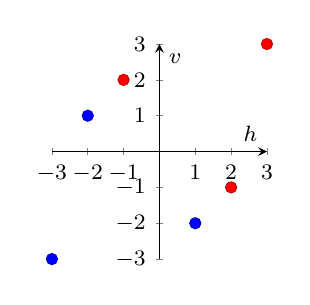
\begin{tikzpicture}
\begin{axis}[footnotesize,font=\footnotesize
    ,xlabel={\(h\)} ,ylabel={\(v\)} ,axis lines=middle
    ,axis equal image]
\addplot[scatter,only marks,scatter src=explicit] 
table[x=x,y=y, meta=S, row sep=\\] {
 x  y S \\
-3 -3 1 \\
-2  1 1 \\
 1 -2 1 \\
-1  2 2 \\
 2 -1 2 \\
 3  3 2 \\
 };
\end{axis}
\end{tikzpicture}}%
\begin{equation*}
\begin{array}{rrp{3em}}
\hline h&v&colour\\\hline
-3&-3&blue \\
-2&1&blue \\
1&-2&blue \\
-1&2&red \\
2&-1&red \\
3&3&red \\\hline
\end{array}
\end{equation*}
The item properties\slash attributes are the points \((h,v)\) in 2D as illustrated in the margin.
But humans always prefer simple one dimensional summaries: we do it all the time when we rank sport teams, schools, web pages, and so on.

Challenge: is there a one dimensional summary of these six item's data that clearly separates the blue from the red?
Using just one of the attributes~\(h\) or~\(v\) on their own would not suffice:
\marginpar{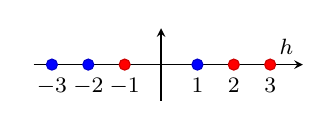
\begin{tikzpicture}
\begin{axis}[footnotesize,font=\footnotesize
    ,xlabel={\(h\)} ,ylabel={}, ytick={0} ,axis lines=middle
    ,axis equal image,xmax=3.9,xmin=-3.5 ]
\addplot[scatter,only marks,scatter src=explicit] 
table[x=x,y=y, meta=S, row sep=\\] {
 x  y S \\
-3  0 1 \\
-2  0 1 \\
 1  0 1 \\
-1  0 2 \\
 2  0 2 \\
 3  0 2 \\
 };
\end{axis}
\end{tikzpicture}}%
\begin{itemize}
\item using \(h\)~alone leads to a 1D view where the red and the blue are intermingled as shown in the margin;
\marginpar{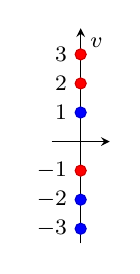
\begin{tikzpicture}
\begin{axis}[footnotesize,font=\footnotesize
    ,xlabel={}, xtick={0} ,ylabel={\(v\)} ,axis lines=middle
    ,axis equal image,ymax=3.9,ymin=-3.5 ]
\addplot[scatter,only marks,scatter src=explicit] 
table[x=x,y=y, meta=S, row sep=\\] {
 x  y S \\
-0 -3 1 \\
-0  1 1 \\
 0 -2 1 \\
-0  2 2 \\
 0 -1 2 \\
 0  3 2 \\
 };
\end{axis}
\end{tikzpicture}}%
\item similarly, using \(v\)~alone leads to a 1D view where the red and the blue are intermingled as shown in the margin.
\end{itemize}

\begin{solution} 
Use an \svd\ to automatically find the best 1D view of the data.
\begin{enumerate}
\item Enter the \(6\times2\) matrix of data into \script\ with
\begin{verbatim}
A=[-3 -3
-2 1
1 -2
-1 2
2 -1
3 3 ]
\end{verbatim}
\setbox\ajrqrbox\hbox{\qrcode{% toy data
A=[-3 -3
-2 1
1 -2
-1 2
2 -1
3 3 ]
[U,S,V]=svd(A)
A*V(:,1)
}}%
\marginpar{\usebox{\ajrqrbox\\[2ex]}}%

\item Then \verb|[U,S,V]=svd(A)| computes an \svd, \(A=\usv\), of the data \twodp:
\begin{verbatim}
U =
  -0.69   0.00  -0.09   0.09   0.14   0.70
  -0.11  -0.50   0.50  -0.50   0.48  -0.08
  -0.11   0.50   0.82   0.18  -0.18   0.01
   0.11  -0.50   0.18   0.82   0.18  -0.01
   0.11   0.50  -0.14   0.14   0.83  -0.09
   0.69  -0.00   0.12  -0.12   0.02   0.70
S =
   6.16      0
      0   4.24
      0      0
      0      0
      0      0
      0      0
V =
   0.71   0.71
   0.71  -0.71
\end{verbatim}

\item Now what does such an \svd\ tell us?
Recall from the proof of the \svd\ (section~\ref{sec:psvdt}) that \(A\vv_1=\sigma_1\uv_1\)\,. 
Further recall from the proof that \(\vv_1\) is the unit vector that maximises~\(|A\vv_1|\) so in some sense it is the direction in which the data in~\(A\) is most spread out (\(\vv_1\)~is called the \idx{principal vector}).
We find here \twodp
\marginpar{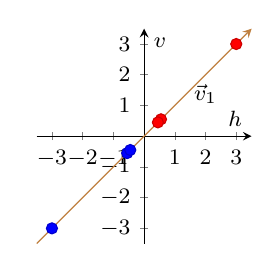
\begin{tikzpicture}
\begin{axis}[footnotesize,font=\footnotesize
    ,xlabel={$h$} ,ylabel={$v$} ,axis lines=middle
    ,axis equal image]
\addplot[scatter,only marks,scatter src=explicit] 
table[x=x,y=y, meta=S, row sep=\\] {
 x  y S \\
  -3.00  -3.00 1 \\
  -0.55  -0.55 1 \\
  -0.45  -0.45 1 \\
   0.55   0.55 2 \\
   0.45   0.45 2 \\
   3.00   3.00 2 \\
 };
\addplot[brown,quiver={u=7,v=7},-stealth]coordinates {(-3.5,-3.5)};
\node[below] at (axis cs:2,2) {$\vec v_1$};
\end{axis}
\end{tikzpicture}}%
\begin{equation*}
A\vv_1=\sigma_1\uv_1=(-4.24,-0.71,-0.71,0.71,0.71,4.24)
\end{equation*}
which neatly separates the blue items (negative) from the red (positive).
In essence, the product~\(A\vv_1\) orthogonally projects (Section~\ref{sec:proj}) the items' \((h,v)\)~data onto the subspace \(\Span\{\vv_1\}\) as illustrated in the margin. 
\end{enumerate}
\end{solution}
\end{example}

Although this Example~\ref{eg:toypca} is just a toy to illustrate concepts, the above steps generalise straightforwardly to be immensely useful on vastly bigger and more challenging data.
The next example takes the next step in complexity by introducing how to automatically find a good 2D view of some data in~4D.





\begin{example}[Iris flower data set] \label{eg:eaid}
\begin{table}
\caption{part of Edgar Anderson's Iris data, lengths in cm.  The measurements come from the flowers of ten each of three different species of Iris.}
\label{tbl:eaid}
\begin{equation*}
\begin{array}{rrrrl}
\hline
\text{Sepal}&\text{Sepal}&\text{Petal}&\text{Petal}&\text{Species}
\\\text{length}&\text{width}&\text{length}&\text{width}&
\\\hline
  4.9&3.0&1.4&0.2&
\\4.6&3.4&1.4&0.3&
\\4.8&3.4&1.6&0.2&
\\5.4&3.9&1.3&0.4&
\\5.1&3.7&1.5&0.4&\text{Setosa}
\\5.0&3.4&1.6&0.4&
\\5.4&3.4&1.5&0.4&
\\5.5&3.5&1.3&0.2&
\\4.5&2.3&1.3&0.3&
\\5.1&3.8&1.6&0.2&
\\\hline
  6.4&3.2&4.5&1.5&
\\6.3&3.3&4.7&1.6&
\\5.9&3.0&4.2&1.5&
\\5.6&3.0&4.5&1.5&
\\6.1&2.8&4.0&1.3&\text{Versicolor}
\\6.8&2.8&4.8&1.4&
\\5.5&2.4&3.7&1.0&
\\6.7&3.1&4.7&1.5&
\\6.1&3.0&4.6&1.4&
\\5.7&2.9&4.2&1.3&
\\\hline
  5.8&2.7&5.1&1.9&
\\4.9&2.5&4.5&1.7&
\\6.4&2.7&5.3&1.9&
\\6.5&3.0&5.5&1.8&
\\5.6&2.8&4.9&2.0&\text{Virginia}
\\6.2&2.8&4.8&1.8&
\\7.9&3.8&6.4&2.0&
\\6.3&3.4&5.6&2.4&
\\6.9&3.1&5.1&2.3&
\\6.3&2.5&5.0&1.9&
\\\hline
\end{array}
\end{equation*}
\end{table}
Table~\ref{tbl:eaid} list part of Edgar Anderson's data on the length and widths of sepals and petals of \idx{Iris} flowers.\footnote{\url{http://archive.ics.uci.edu/ml/datasets/Iris} gives the full dataset \cite[]{Lichman2013}.}
There are three \idx{species} of Irises in the data (Setosa, Versicolor, Virginia).
The data is 4D: each instance of thirty Iris flowers is characterised by the four measurements of sepals and petals.
Our challenge is to plot a 2D picture of this data in such a way that separates the flowers as best as possible.
For high-D data (although 4D is not really that high), simply plotting one characteristic against another is rarely useful.
For example,  Figure~\ref{fig:eaid} plots the attributes of sepal widths versus sepal lengths: the plot shows the three species being intermingled together rather than reasonably separated.
Our aim is to instead plot Figure~\ref{fig:eaidpca} which successfully separates the three species.

\begin{figure}
\centering
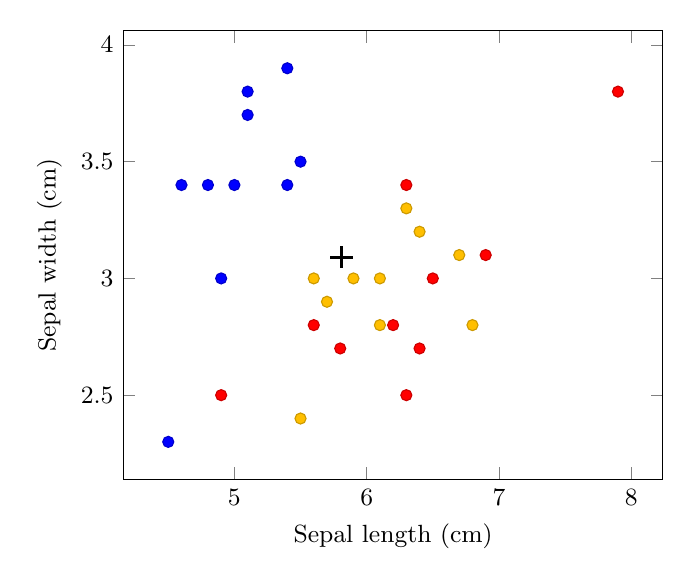
\begin{tikzpicture}
\begin{axis}[font=\small
    ,xlabel={Sepal length (cm)}
    ,ylabel={Sepal width (cm)}]
\addplot[scatter,only marks,scatter src=explicit] 
table[x=SeL,y=SeW, meta=S] {
 SeL SeW PeL PeW S
 4.9 3.0 1.4 0.2 1
 4.6 3.4 1.4 0.3 1
 4.8 3.4 1.6 0.2 1
 5.4 3.9 1.3 0.4 1
 5.1 3.7 1.5 0.4 1
 5.0 3.4 1.6 0.4 1
 5.4 3.4 1.5 0.4 1
 5.5 3.5 1.3 0.2 1
 4.5 2.3 1.3 0.3 1
 5.1 3.8 1.6 0.2 1
 6.4 3.2 4.5 1.5 2
 6.3 3.3 4.7 1.6 2
 5.9 3.0 4.2 1.5 2
 5.6 3.0 4.5 1.5 2
 6.1 2.8 4.0 1.3 2
 6.8 2.8 4.8 1.4 2
 5.5 2.4 3.7 1.0 2
 6.7 3.1 4.7 1.5 2
 6.1 3.0 4.6 1.4 2
 5.7 2.9 4.2 1.3 2
 5.8 2.7 5.1 1.9 3
 4.9 2.5 4.5 1.7 3
 6.4 2.7 5.3 1.9 3
 6.5 3.0 5.5 1.8 3
 5.6 2.8 4.9 2.0 3
 6.2 2.8 4.8 1.8 3
 7.9 3.8 6.4 2.0 3
 6.3 3.4 5.6 2.4 3
 6.9 3.1 5.1 2.3 3
 6.3 2.5 5.0 1.9 3
};
\addplot[black,mark=+,mark size=4,thick] coordinates {(5.81,3.09)};
\end{axis}
\end{tikzpicture}
\caption{scatter plot of sepal widths versus lengths for Edgar Anderson's iris data of Table~\ref{tbl:eaid}: blue,~Setosa; brown,~Versicolor; red,~Virginia.  
The black~``+'' marks the mean sepal width and length.}
\label{fig:eaid}
\end{figure}

\begin{solution} 
Use an \svd\ to find a best low-rank view of the data.
\begin{enumerate}
\item Enter the \(30\times5\) matrix of Iris data into \script\  with a complete version of
\begin{verbatim}
iris=[
4.9 3.0 1.4 0.2 1
4.6 3.4 1.4 0.3 1
...
6.3 2.5 5.0 1.9 3
]
\end{verbatim}
where the fifth column of~\(1,2,3\) corresponds to the species Setosa, Versicolor or Virginia, respectively.
\setbox\ajrqrbox\hbox{\qrcode{% Iris data
iris=[
4.9 3.0 1.4 0.2 1
4.6 3.4 1.4 0.3 1
4.8 3.4 1.6 0.2 1
5.4 3.9 1.3 0.4 1
5.1 3.7 1.5 0.4 1
5.0 3.4 1.6 0.4 1
5.4 3.4 1.5 0.4 1
5.5 3.5 1.3 0.2 1
4.5 2.3 1.3 0.3 1
5.1 3.8 1.6 0.2 1
6.4 3.2 4.5 1.5 2
6.3 3.3 4.7 1.6 2
5.9 3.0 4.2 1.5 2
5.6 3.0 4.5 1.5 2
6.1 2.8 4.0 1.3 2
6.8 2.8 4.8 1.4 2
5.5 2.4 3.7 1.0 2
6.7 3.1 4.7 1.5 2
6.1 3.0 4.6 1.4 2
5.7 2.9 4.2 1.3 2
5.8 2.7 5.1 1.9 3
4.9 2.5 4.5 1.7 3
6.4 2.7 5.3 1.9 3
6.5 3.0 5.5 1.8 3
5.6 2.8 4.9 2.0 3
6.2 2.8 4.8 1.8 3
7.9 3.8 6.4 2.0 3
6.3 3.4 5.6 2.4 3
6.9 3.1 5.1 2.3 3
6.3 2.5 5.0 1.9 3
];
}}%
\marginpar{\usebox{\ajrqrbox\\[2ex]}}%
Then a scatter plot such as Figure~\ref{fig:eaid} may be drawn with the command
\begin{verbatim}
scatter(iris(:,1),iris(:,2),[],iris(:,5))
\end{verbatim}
The above command \index{scatter()@\texttt{scatter()}}\verb|scatter(x,y,[],s)|  plots a scatter plot of points with colour depending upon~\verb|s| which here corresponds to each different species.

\item If we were on a walk to a scenic lookout to get a view of the countryside, then the scenic lookout would be in the countryside: it is no good going to a lookout a long way away from the scene we wish to view.
Correspondingly, to best view a dataset we typically look it at from the very centre of the data, namely its mean.
That is, here we use an \svd\ of the data matrix only after subtracting the mean of each attribute so that the \svd\ analyses the variations from the mean.
Here the mean Iris sepal length and width is \(5.81\)\,cm and~\(3.09\)\,cm (the black~``+'' in Figure~\ref{fig:eaid}), and the mean petal length and width is \(3.69\)\,cm and~\(1.22\)\,cm.
In \script\ execute the following to form a matrix~\(A\) of the variations from the mean, and compute an \svd:
\begin{verbatim}
meaniris=mean(iris(:,1:4))
A=iris(:,1:4)-ones(30,1)*meaniris
[U,S,V]=svd(A)
\end{verbatim}
\setbox\ajrqrbox\hbox{\qrcode{% view Iris
meaniris=mean(iris(:,1:4))
A=iris(:,1:4)-ones(30,1)*meaniris
[U,S,V]=svd(A)
scatter(A*V(:,1),A*V(:,2),[],iris(:,5))
}}%
\marginpar{\usebox{\ajrqrbox\\[2ex]}}%
The resulting \svd\ is \twodp
\begin{verbatim}
U = ...
S =
   10.46       0       0       0
       0    2.86       0       0
       0       0    1.47       0
       0       0       0    0.85
      ...     ...     ...     ...
V =
   0.34   0.72  -0.56  -0.20
  -0.07   0.65   0.74   0.14
   0.87  -0.17   0.14   0.45
   0.36  -0.15   0.33  -0.86
\end{verbatim}
where a \verb|...| indicates information that is not directly of interest.

\begin{figure}
\centering
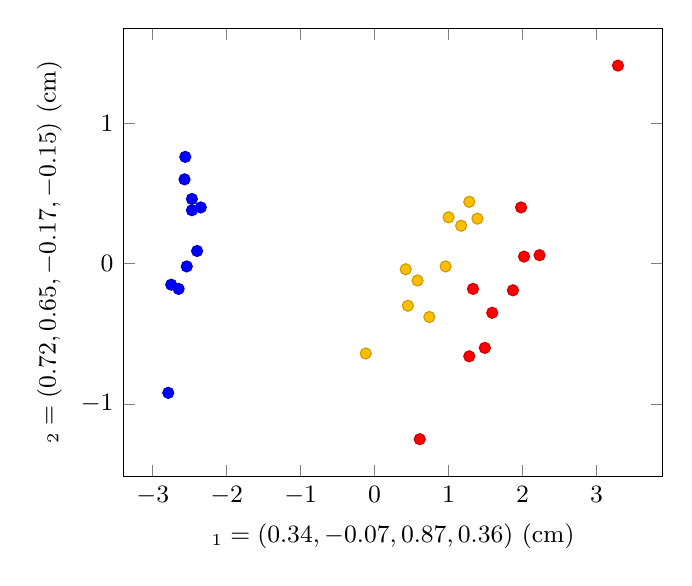
\begin{tikzpicture}
\begin{axis}[font=\small
    ,xlabel={$\vv_1=(0.34,-0.07,0.87,0.36)$ (cm)}
    ,ylabel={$\vv_2=(0.72,0.65,-0.17,-0.15)$ (cm)}]
\addplot[scatter,only marks,scatter src=explicit] 
table[x=x,y=y, meta=S] {
   x     y    S
 -2.65 -0.18  1
 -2.75 -0.15  1
 -2.54 -0.02  1
 -2.56  0.76  1
 -2.47  0.38  1
 -2.40  0.09  1
 -2.35  0.40  1
 -2.57  0.60  1
 -2.79 -0.92  1
 -2.47  0.46  1
  1.00  0.33  2
  1.17  0.27  2
  0.58 -0.12  2
  0.74 -0.38  2
  0.42 -0.04  2
  1.39  0.32  2
 -0.12 -0.64  2
  1.28  0.44  2
  0.96 -0.02  2
  0.45 -0.30  2
  1.49 -0.60  3
  0.61 -1.25  3
  1.87 -0.19  3
  2.02  0.05  3
  1.28 -0.66  3
  1.33 -0.18  3
  3.29  1.41  3
  2.23  0.06  3
  1.98  0.40  3
  1.59 -0.35  3
};
\end{axis}
\end{tikzpicture}
\caption{best 2D scatter plot of Edgar Anderson's iris data: blue,~Setosa; brown,~Versicolor; red,~Virginia. }
\label{fig:eaidpca}
\end{figure}%
\item As justified shortly, the two most important components of a flower's shape are those in the directions of~\(\vv_1\) and~\(\vv_2\) (called the two \idx{principal vector}s).
Because \(\vv_1\) and~\(\vv_2\) are orthonormal, the first component for each Iris flower is \(\xv=A\vv_1\) and the second component for each is \(\yv=A\vv_2\)\,.
The beautiful Figure~\ref{fig:eaidpca} is a scatter plot of the components of~\yv\ versus the components of~\xv\ that untangles the three species.
Obtain Figure~\ref{fig:eaidpca} in \script\ with the command
\begin{verbatim}
scatter(A*V(:,1),A*V(:,2),[],iris(:,5))
\end{verbatim}
Figure~\ref{fig:eaidpca} shows our \svd\ based analysis largely separates the three species using these two different combinations of the flowers' attributes.
\end{enumerate}
\end{solution}
\end{example}




\paragraph{Transpose the usual mathematical convention}
Perhaps you noticed that the previous Example~\ref{eg:eaid} flips our usual mathematical convention that vectors are column vectors.
The example uses \idx{row vector}s of the four attributes of each flower: 
Table~\ref{tbl:eaid} lists that the first Iris Setosa flower has a row vector of attributes \(\begin{bmatrix} 4.9&3.0&1.4&0.2 \end{bmatrix}\)~(cm) corresponding to the sepal length and width, and the petal length and width, respectively.
Similarly, the last Virginia Iris flower has row vector of attributes of \(\begin{bmatrix} 46.3&2.5&5.0&1.9 \end{bmatrix}\)~(cm), and the mean vector is the row vector \(\begin{bmatrix} 5.81&3.09&3.69&1.22 \end{bmatrix}\)~(cm).
The reason for this mathematical transposition is that throughout science and engineering, data results are most often presented as rows of different instances of flowers, animals, clients or experiments: each row contains the list of characteristic measured or derived properties\slash attributes.
Table~\ref{tbl:eaid} has this most common structure.
Thus in this sort of application, the mathematics we do needs to reflect this most common structure.
Hence many vectors in this subsection appear as row vectors.




\begin{definition}[principal components] \label{def:}
Given a \(m\times n\) data matrix~\(A\) (usually with zero mean when averaged over all rows),  with  \svd\ \(A=\usv\) the \(j\)th column~\(\vv_j\) of~\(V\) is called the \(j\)th~\bfidx{principal vector} and the vector \(\xv_j:=A\vv_j\) is called the \(j\)th~\bfidx{principal components} of the data matrix~\(A\).
\end{definition}



Now what does an \svd\ tell us for 2D plots of data?  
We know \(A_2\) is the best rank two approximation to the data matrix~\(A\) (Theorem~\ref{thm:am}). 
That is, if we are only to plot two components, those two components are best to come from~\(A_2\).
Recall from~\eqref{eq:rankkA} that
\begin{equation*}
A_2=US_2\tr V =\sigma_1\uv_1\tr\vv_1 +\sigma_2\uv_2\tr\vv_2
=(\sigma_1\uv_1)\tr\vv_1 +(\sigma_2\uv_2)\tr\vv_2\,.
\end{equation*}
That is, in this best rank two approximation of the data, the row vector of attributes of the \(i\)th~Iris are the linear combination of row vectors \((\sigma_1u_{i1})\tr\vv_1+(\sigma_2u_{i2})\tr\vv_2\).
The vectors \(\vv_1\) and~\(\vv_2\) are orthonormal vectors so we treat them as the horizontal and vertical unit vectors of a scatter plot. 
That is, \(x_i=\sigma_1u_{i1}\) and \(y_i=\sigma_2u_{i2}\) are horizontal and vertical coordinates of the \(i\)th~Iris in the best 2D plot.
Consequently, in \script\ we draw a scatter plot of the components of vectors \(\xv=\sigma_1\uv_1\) and \(\yv=\sigma_2\uv_2\) (Figure~\ref{fig:eaidpca}).


\begin{theorem} \label{thm:}
Using the \idx{matrix norm} to measure `best', the best \(k\)-dimensional summary of the \(m\times n\) data matrix~\(A\)  (usually of zero mean) are the first~\(k\) principal components in the directions of the first~\(k\) principal vectors.
\end{theorem}

\begin{proof} 
Let \(A=\usv\) be an \svd\ of matrix~\(A\).
For every \(k<\rank A\), Theorem~\ref{thm:am} establishes that 
\begin{equation*}
A_k:=US_k\tr V 
=\sigma_1\uv_1\tr\vv_1 +\sigma_2\uv_2\tr\vv_2+\cdots +\sigma_k\uv_k\tr\vv_k
\end{equation*}
is the best rank~\(k\) approximation to~\(A\) in the matrix norm.
Letting matrix \(U=\begin{bmatrix} u_{ij} \end{bmatrix}\), write the \(i\)th~row of~\(A_k\) as
\((\sigma_1u_{i1})\tr\vv_1 +(\sigma_2u_{i2})\tr\vv_2+\cdots +(\sigma_ku_{ik})\tr\vv_k\) and hence the transpose of each row of~\(A_k\) lies in the \(k\)D~subspace \(\Span\{\hlist\vv k\}\).
This establishes that these are principal vectors.

Since \(\{\hlist\vv k\}\) is an orthonormal set, we now use them as standard unit vectors of a coordinate system for the \(k\)D~subspace.
From the above linear combination, the components of the \(i\)th~data point approximation in this subspace coordinate system are \(\sigma_1u_{i1},\sigma_2u_{i2},\ldots,\sigma_ku_{ik}\).
That is, the \(j\)th~coordinate for all data points, the principal components, is~\(\sigma_j\uv_j\).
By post-multiplying the \svd\ \(A=\usv\) by orthogonal~\(V\), recall that \(AV=US\) which written in terms of columns is
\begin{equation*}
\begin{bmatrix} A\vv_1&A\vv_2&\cdots&A\vv_r \end{bmatrix}
=\begin{bmatrix} \sigma_1\uv_1&\sigma_2\uv_2&\cdots&\sigma_r\uv_mr\end{bmatrix}
\end{equation*}
where \(r=\rank A\)\,.  
Consequently, the vector~\(\sigma_j\uv_j\) of \(j\)th~coordinates in the subspace are equal to~\(A\vv_j\), the principal components.
\end{proof}




\begin{activity}
A given data matrix from some experiment has singular values \(12.76\), \(10.95\), \(7.62\), \(0.95\), \(0.48\), \ldots.  How many dimensions should be needed for a good view of the data?
\partswidth=5em
\begin{parts}
\item 1D
\item 2D
\item 3D
\item 4D
\end{parts}
\end{activity}






\begin{example}[\idx{wine recognition}] \label{eg:winepca}
From the \cite{Lichman2013} repository\footnote{\url{http://archive.ics.uci.edu/ml/datasets/Wine}} download the data file \verb|wine.data| and its description file \verb|wine.names|.
The wine data has 178~rows of different wine samples, and 14~columns of attributes of which the first column is the cultivar class number and the remaining 13~columns are the amounts of different chemicals measured in the wine.
Question: is there a two-dimensional view of these chemical measurements that largely separates the cultivars?

\begin{solution} 
Use an \svd\ to find the best two-dimensional, rank two, view of the data.
\begin{enumerate}
\item Read in the \(178\times14\) matrix of data into \script\ with the commands\index{csvread()@\texttt{csvread()}}
\begin{verbatim}
wine=csvread('wine.data')
[m,n]=size(wine)
scatter(wine(:,2),wine(:,3),[],wine(:,1))
\end{verbatim}
\setbox\ajrqrbox\hbox{\qrcode{% view wine
wine=csvread('wine.data')
[m,n]=size(wine)
scatter(wine(:,2),wine(:,3),[],wine(:,1))
meanw=mean(wine(:,2:14))
stdw=std(wine(:,2:14))
A=(wine(:,2:14)-ones(m,1)*meanw)*diag(1./stdw);
[U,S,V]=svds(A,4)
scatter(A*V(:,1),A*V(:,2),[],wine(:,1))
}}%
\marginpar{\usebox{\ajrqrbox\\[2ex]}}%
The scatter plot, Figure~\ref{fig:wine12}, shows that if we just plot the first two chemicals, alcohol and malic acid, then the three cultivars are inextricably intermingled.
Our aim is to automatically draw Figure~\ref{fig:winepca} in which the three cultivars are largely separated.
\begin{figure}
\centering
\input{ApproxMat/wine12.ltx}
\caption{for the wine data of Example~\ref{eg:winepca}, a plot of the measured malic acid versus measured alcohol, and coloured depending upon the cultivar, shows these measurements alone cannot effectively discriminate between the cultivars.}
\label{fig:wine12}
\end{figure}


\item To find the principal components of the wine chemicals it is best to remove the mean with
\begin{verbatim}
meanw=mean(wine(:,2:14))
A=wine(:,2:14)-ones(m,1)*meanw;
\end{verbatim}
where the \index{mean()@\texttt{mean()}}\verb|mean(X)| computes the \idx{mean}\slash \idx{average} of each column of~\verb|X|.

But now a further issue arises: the values in the columns are of widely different magnitudes; moreover, each column has different physical units (in contrast, the Iris flower measurements were all cm).
In practice we \emph{must not} mix together quantities with different physical units. 
The general rule, after making each column zero mean, is to \index{data scaling}scale each column by dividing by its \idx{standard deviation},  equivalently by its root-mean-square.
This scaling does two practically useful things: 
\begin{itemize}
\item since the standard deviation measures the spread of data in a column, it has the same physical units as the column of data, so dividing by it renders the results dimensionless, and so suitable for mixing with other scaled columns;
\item also the spread of data in each column is now comparable to each other, namely around about size one, instead of some columns being of the order of one-tenths and other columns being in the hundreds.
\end{itemize}
Consequently, form the \(178\times13\) matrix to analyse by commands
\begin{verbatim}
meanw=mean(wine(:,2:14))
stdw=std(wine(:,2:14))
A=(wine(:,2:14)-ones(m,1)*meanw)*diag(1./stdw);
\end{verbatim}
where the \index{std()@\texttt{std()}}\verb|std(X)| computes the \idx{standard deviation} of each column of~\verb|X|.

\item Now compute and use an \svd\ \(A=\usv\).
But for low rank approximations we only ever use the first few singular values and first few singular vectors.
Thus it is pointless computing a full \svd\ which here has \(178\times178\) matrix~\(U\) and \(13\times13\) matrix~\(V\).\footnote{Yes, on modern computers this is here done within a millisecond.  But for modern datasets with thousands to billions of rows a full \svd\ is infeasible so let's see how to analyse such modern large datasets.}
Consequently, use \index{svds()@\texttt{svds()}}\verb|[U,S,V]=svds(A,4)| to economically compute only the first four singular values and singular vectors (change the four to suit your purpose) to find \twodp
\begin{verbatim}
U = ...
S =
   28.86       0       0       0
       0   21.02       0       0
       0       0   16.00       0
       0       0       0   12.75
V =
  -0.14   0.48  -0.21  -0.02
   0.25   0.22   0.09   0.54
   0.00   0.32   0.63  -0.21
   0.24  -0.01   0.61   0.06
  -0.14   0.30   0.13  -0.35
  -0.39   0.07   0.15   0.20
  -0.42  -0.00   0.15   0.15
   0.30   0.03   0.17  -0.20
  -0.31   0.04   0.15   0.40
   0.09   0.53  -0.14   0.07
  -0.30  -0.28   0.09  -0.43
  -0.38  -0.16   0.17   0.18
  -0.29   0.36  -0.13  -0.23
\end{verbatim}
where the \verb|...| indicates we do not here need to know~\(U\).

\item Recall that the columns of this orthogonal~\(V\) are the principal vectors \hlist\vv 4, and the \(j\)th~principal components of the data are \(\xv_j=A\vv_j\)\,.
We form a 2D plotted view of the data, Figure~\ref{fig:winepca}, by drawing a scatter plot of the first two principal components with 
\begin{verbatim}
scatter(A*V(:,1),A*V(:,2),[],wine(:,1))
\end{verbatim}
\begin{figure}
\centering
\input{ApproxMat/wine2d.ltx}\\
\caption{for the wine data of Example~\ref{eg:winepca}, a plot of the first two principal components almost entirely separates the three cultivars.}
\label{fig:winepca}
\end{figure}
\end{enumerate}
Figure~\ref{fig:winepca} shows these two principal components do an amazingly good job of almost completely disentangling the three wine cultivars (use \verb|scatter3()| to explore the first three principal components).
\end{solution}
\end{example}


The previous three examples develop the following procedure for `best' viewing data in low dimensions.
%The procedure is automatic.
However, any additional information about the data or preferred results may modify this procedure. 


\begin{procedure}[principal component analysis] \label{pro:pca}
Consider the case when you have data values consisting of \(n\)~attributes for each of \(m\)~instances, and the aim is to find a good \(k\)-dimensional summary\slash view of the data. 
\begin{enumerate}
\item Form\slash enter the \(m\times n\) data matrix~\(B\).
\item \index{data scaling}Scale the data matrix~\(B\) to form \(m\times n\) matrix~\(A\):
\begin{enumerate}
\item usually make each column have zero mean by subtracting its mean~\(\bar b_j\), algebraically \(\av_j=\bv_j-\bar b_j\)\,;
\item but ensure each column has the same `physical dimensions', often by dividing by the \idx{standard deviation}~\(s_j\) of each column, algebraically \(\av_j=(\bv_j-\bar b_j)/s_j\)\,.
\end{enumerate}
Compute \verb|A=(B-ones(m,1)*mean(B))*diag(1./std(B))| in \script.
\item  Economically compute an \svd\ for the best rank~\(k\) approximation to the scaled data matrix with \index{svds()@\texttt{svds()}}\verb|[U,S,V]=svds(A,k)|.
\item Then the \(j\)th~column of~\verb|V| is the \(j\)th~\idx{principal vector}, and the \idx{principal components} are the entries of the \(m\times k\) matrix~\verb|A*V|.
\end{enumerate}
\end{procedure}




Courses on multivariate statistics prove that, for every (usually zero mean) data matrix~\(A\), the first~\(k\) principal vectors \hlist\vv k\ are orthogonal unit vectors that \emph{maximise the total \idx{variance}} in the principal components \(\xv_j=A\vv_j\)\,; that is, that maximise \(|\xv_1|^2+|\xv_2|^2+\cdots+|\xv_k|^2\).
Indeed, this maximisation of the variance corresponds closely to the constructive proof of the existence of \svd{}s (section~\ref{sec:psvdt}) which successively maximises~\(|A\vv|\) subject to~\vv\ being orthonormal to the singular\slash principal vectors already determined.
Consequently, when data is approximated in the space of the first~\(k\) principal vectors, then the data is the most spread out it can be in \(k\)-dimensions.


\index{principal vector|)}
\index{principal components|)}





\subsubsection{Application to latent semantic indexing}
\label{sec:alsi}
\index{latent semantic indexing|(}
%\begin{example}[\idx{latent semantic indexing}] \label{eg:bktitlepca}

\begin{quoted}{\cite[p.579]{Berry95}}
This ability to retrieve relevant information based upon meaning rather than literal term usage is the main motivation for using \textsc{lsi} [latent semantic indexing].
\end{quoted}

Searching for information based upon word matching results in surprisingly poor retrieval of relevant documents \cite[\S5.5]{Berry95}.
Instead, the so-called method of latent semantic indexing improves retrieval by replacing individual words with nearness of word vectors derived via the singular value decomposition.
This section introduces latent semantic indexing via a very small example. 


The Society for Industrial and Applied Mathematics (\textsc{siam}) reviews many mathematical books.
In 2015 six of those books had the following titles:
\begin{enumerate}
\item Introduction to Finite and Spectral Element Methods using \textsc{matlab}
\item Iterative Methods for Linear Systems: Theory and Applications 
\item Singular Perturbations: Introduction to System Order Reduction Methods with Applications 
\item Risk and Portfolio Analysis: Principles and Methods 
\item Stochastic Chemical Kinetics: Theory and Mostly Systems Biology Applications
\item Quantum Theory for Mathematicians 
\end{enumerate}
Consider the capitalised words. 
For those words that appear in more than one title, let's form a \idx{word vector} (Example~\ref{eg:deflsv}) for each title, then use \idx{principal components} to summarise these six books on a 2D~plane.
This task is part of what is called \idx{latent semantic indexing} \cite[]{Berry95}.  
(We should also count words that are used only once, but this example omits for simplicity.)

%Useful in LSI is\\
%\verb#tr -cs "[:alpha:]" "\n" < books.txt |sort -f#
%\verb#head file -20|tr -cs "[:alpha:]" "\n"|sort -f#

Follow the \idx{principal component analysis} Procedure~\ref{pro:pca}.
\begin{enumerate}
\item 
First find the set of words that are used more than once.
Ignoring pluralisation, they are: 
Application, Introduction, Method, System, Theory.
The corresponding \idx{word vector} for each book title is then the following:
\begin{itemize}
\item \(\wv_1=(0,1,1,0,0)\) \emph{Introduction} to Finite and Spectral Element \emph{Method}s using \textsc{matlab}
\item \(\wv_2=(1,0,1,1,1)\) Iterative \emph{Method}s for Linear \emph{System}s: \emph{Theory} and \emph{Application}s 
\item \(\wv_3=(1,1,1,1,0)\) Singular Perturbations: \emph{Introduction} to \emph{System} Order Reduction \emph{Method}s with \emph{Application}s 
\item \(\wv_4=(0,0,1,0,0)\) Risk and Portfolio Analysis: Principles and \emph{Method}s 
\item \(\wv_5=(1,0,0,1,1)\) Stochastic Chemical Kinetics: \emph{Theory} and Mostly \emph{System}s Biology \emph{Application}s
\item \(\wv_6=(0,0,0,0,1)\) Quantum \emph{Theory} for Mathematicians 
\end{itemize}

\item Second, form the data matrix with \hlist\wv 6\ as rows (not columns).
We could remove the mean word vector, but choose not to: here the position of each book title relative to an empty title (the origin) is interesting.
There is no need to \index{data scaling}scale each column as each column has the same `physical' dimensions, namely a word count.
The data matrix of word vectors is then
\begin{equation*}
A=\begin{bmatrix} 0&1&1&0&0
\\1&0&1&1&1
\\1&1&1&1&0
\\0&0&1&0&0
\\1&0&0&1&1
\\0&0&0&0&1 \end{bmatrix}.
\end{equation*}
\setbox\ajrqrbox\hbox{\qrcode{% latent semantic indexing
A=[0 1 1 0 0
 1 0 1 1 1
 1 1 1 1 0
 0 0 1 0 0
 1 0 0 1 1
 0 0 0 0 1 ]
[U,S,V]=svds(A,2)
scatter(A*V(:,1),A*V(:,2),[],1:6)
}}%
\marginpar{\usebox{\ajrqrbox\\[2ex]}}%


\item Third, to compute a representation in the 2D plane, principal components uses, as an \idx{orthonormal basis}, the singular vectors corresponding to the two largest singular values.  
So compute the economical \svd\ with \index{svds()@\texttt{svds()}}\verb|[U,S,V]=svds(A,2)| giving \twodp
\begin{verbatim}
U = ...
S =
   3.14      0
      0   1.85
V =
  +0.52  -0.20
  +0.26  +0.52
  +0.50  +0.57
  +0.52  -0.20
  +0.37  -0.57
\end{verbatim}

\item Columns of~\(V\) are word vectors in the 5D space of counts of Application, Introduction, Method, System, and Theory.
The two given columns of \(V=\begin{bmatrix} \vv_1&\vv_2 \end{bmatrix}\) are the two orthonormal \idx{principal vector}s:
\begin{itemize}
\item the first~\(\vv_1\), from its largest components, mainly identifies the overall direction of Application, Method and System;
\item whereas the second~\(\vv_2\), from its largest positive and negative components, mainly distinguishes Introduction and Method from Theory.
\end{itemize}
The corresponding \idx{principal components} are the entries of the \(6\times 2\) matrix
\begin{equation*}
AV=\begin{bmatrix} 0.76 & 1.09 \\
1.92 & -0.40 \\
1.80 & 0.69 \\
0.50 & 0.57 \\
1.41 & -0.97 \\
0.37 & -0.57 \end{bmatrix}:
\end{equation*}
for each of the six books, the book title has components in the two principal directions given by the corresponding row in this product.
\marginpar{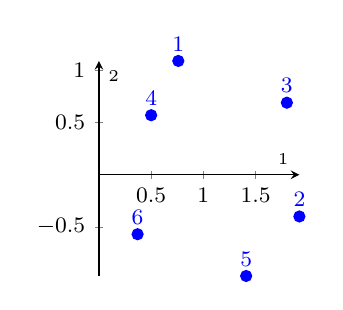
\begin{tikzpicture}
\begin{axis}[footnotesize,font=\footnotesize
  ,nodes near coords, xmin=0, axis lines=middle,axis equal image
  ,xlabel={$\vv_1$},ylabel={$\vv_2$}]
\addplot+[scatter,only marks,scatter src=explicit] 
table[x=x,y=y, meta=s,row sep=\\] {
 x y s \\
   0.76   1.09   1 \\
   1.92  -0.40   2 \\
   1.80   0.69   3 \\
   0.50   0.57   4 \\
   1.41  -0.97   5 \\
   0.37  -0.57   6 \\
};
\end{axis}
\end{tikzpicture}}
We plot the six books on a 2D~plane with the \script\ command
\begin{verbatim}
scatter(A*V(:,1),A*V(:,2),[],1:6)
\end{verbatim}
to produce a picture like that in the margin.
The \svd\ analysis nicely distributes the books in this plane.
\end{enumerate}

The above procedure would approximate the original word vector data, formed into a matrix, by the following rank two matrix \twodp
\begin{equation*}
A_2=US_2\tr V
=\begin{bmatrix} 0.18&0.77&1.01&0.18&-0.33
\\1.08&0.29&0.74&1.08&0.95
\\0.80&0.82&1.30&0.80&0.28
\\0.15&0.43&0.58&0.15&-0.14
\\0.93&-0.14&0.16&0.93&1.08
\\0.31&-0.20&-0.14&0.31&0.46 \end{bmatrix}.
\end{equation*}
The largest components in each row do correspond to the ones in the original word vector matrix~\(A\).
However, in this application we work with the representation in the low dimensional,~2D, subspace spanned by the first two principal vectors~\(\vv_1\) and~\(\vv_2\).


\paragraph{Angles measure similarity}
Recall that Example~\ref{eg:lsidot} introduced using the \idx{dot product} to measure the similarity between word vectors.
We could use the dot product in the 5D~space of the word vectors to find the `angles' between the book titles.
However, we know that the 2D~view just plotted is the `best' 2D~summary of the book titles, so we could more economically estimate the angle between book titles using just the 2D~summary.

\begin{example} \label{eg:}
What is the `angle' between the first two listed books?
\begin{itemize}
\item Introduction to Finite and Spectral Element Methods using \textsc{matlab}
\item Iterative Methods for Linear Systems: Theory and Applications 
\end{itemize}
\begin{solution} 
Find the angle two ways.
\begin{enumerate}
\item First, the corresponding 5D word vectors are \(\wv_1=(0,1,1,0,0)\) and \(\wv_2=(1,0,1,1,1)\), with lengths \(|\wv_1|=\sqrt2\) and \(|\wv_2|=\sqrt4=2\)\,.
The dot product then determines
\begin{equation*}
\cos\theta=\frac{\wv_1\cdot\wv_2}{|\wv_1|\,|\wv_2|}
=\frac{0+0+1+0+0}{2\sqrt2} =0.3536\,.
\end{equation*}
Hence the angle \(\theta=69.30^\circ\).
\item Secondly, estimate the angle using the 2D~view.
For these two books the principal component vectors are \((0.76,1.09)\) and \((1.92,-0.40)\), respectively, with lengths~\(1.33\) and~\(1.96\) \twodp.
The dot product gives
\begin{equation*}
\cos\theta\approx \frac{(0.76,1.09)\cdot(1.92,-0.40)}{1.33\cdot 1.96}
= \frac{1.02}{2.61}=0.39\,.
\end{equation*}
Hence the angle \(\theta\approx67^\circ\) which is effectively the same as the first exact calculation.
\end{enumerate}
Because of the relatively large `angle' between these two book titles, we deduce that the two books are quite dissimilar.
\end{solution}
\end{example}

We can also use the 2D~plane to economically measure similarity between the book titles and any other title or words of interest.

\begin{example} \label{eg:bks6q}
Let's ask which of the six books is `closest' to a book about Applications.
\begin{solution} 
The word Application has word vector \(\wv=(1,0,0,0,0)\).
So we could do some computations in the original 5D~space of word vectors finding precise angles between this word vector and the word vectors of all titles.
Alternatively, let's draw a picture in~2D.
The Application word vector~\wv\ projects onto the 2D~plane of principal components by computing \(\wv\cdot\vv_1=\tr\wv\vv_1\) and \(\wv\cdot\vv_2=\tr\wv\vv_2\), that is, \(\tr\wv V\).
Here the Application word vector \(\wv=(1,0,0,0,0)\), so \(\tr\wv V=\begin{bmatrix} 0.52 & -0.20 \end{bmatrix}\), as plotted in the margin.
\marginpar{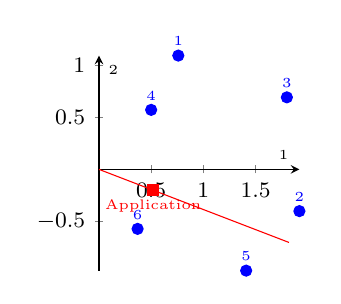
\begin{tikzpicture}
\begin{axis}[footnotesize,font=\tiny
  , xmin=0, axis lines=middle,axis equal image
  ,xlabel={$\vv_1$},ylabel={$\vv_2$}]
\addplot+[scatter,only marks,scatter src=explicit,nodes near coords] 
table[x=x,y=y, meta=s,row sep=\\] {
 x y s \\
   0.76   1.09   1 \\
   1.92  -0.40   2 \\
   1.80   0.69   3 \\
   0.50   0.57   4 \\
   1.41  -0.97   5 \\
   0.37  -0.57   6 \\
};
\addplot+[only marks,forget plot] coordinates {(0.52,-0.20)} 
node[below] {Application};
\addplot+[domain=0:3.5,no marks] ({0.52*\x},{-0.20*\x});
\end{axis}
\end{tikzpicture}}
Which of the six books makes the smallest angle with the line through \((0.52,-0.20)\)?
Visually, books~2 and~5 are closest, and book~2 appears to have slightly smaller angle to the line than book~5.
On this data, we deduce that closest to ``Application'' is book~2: ``Iterative Methods for Linear Systems: Theory and Applications''
\end{solution}
\end{example}






\paragraph{Search for information from more books}
\cite{Berry95} reviewed the application of the \svd\ to the problem of \idx{searching} for information.
Let's explore this further with more data, albeit still very restricted.
\cite{Berry95} listed some mathematical books including the following fourteen titles.
\begin{enumerate}
\item a Course on Integral Equations
\item Automatic Differentiation of Algorithms: Theory, Implementation, and Application
\item Geometrical Aspects of Partial Differential Equations
\item Introduction to Hamiltonian Dynamical Systems and the n-Body Problem
\item Knapsack Problems: Algorithms and Computer Implementations 
\item Methods of Solving Singular Systems of Ordinary Differential Equations
\item Nonlinear Systems
\item Ordinary Differential Equations
\item Oscillation Theory of Delay Differential Equations 
\item Pseudodifferential Operators and Nonlinear Partial Differential Equations
\item Sinc Methods for Quadrature and Differential Equations 
\item Stability of Stochastic Differential Equations with Respect to Semi-Martingales
\item the Boundary Integral Approach to Static and Dynamic Contact Problems
\item the Double Mellin--Barnes Type Integrals and their Applications to Convolution Theory
\end{enumerate}
Principal component analysis summarises and relates these titles.
\def\temp#1{%
\begin{center}
\def\threevcol{red}
\qview{25}{29} {\begin{tikzpicture}
\begin{axis}[normalsize,font=\footnotesize
  , axis equal image,view={\q}{30}
  ,xmin=0,xmax=1.9,ymin=-0.5,ymax=1.7,zmin=-1.5,zmax=1.1
  ,xlabel={$\vv_1$},ylabel={$\vv_2$},zlabel={$\vv_3$},label shift={-2ex}]
\addplot3+[scatter,only marks,scatter src=explicit,nodes near coords] 
table[x=x,y=y,z=z, meta=s,row sep=\\] {
 x y z s \\
    0.70    0.09   -0.25    1 \\
    1.02    1.59    1.00    2 \\
    1.46   -0.29    0.10    3 \\
    0.16    0.67   -1.44    4 \\
    0.16    1.19   -0.22    5 \\
    1.78   -0.34   -0.64    6 \\
    0.22   -0.00   -0.58    7 \\
    1.48   -0.29   -0.04    8 \\
    1.45    0.21    0.40    9 \\
    1.56   -0.34   -0.01   10 \\
    1.48   -0.29   -0.04   11 \\
    1.29   -0.20    0.08   12 \\
    0.10    0.92   -1.14   13 \\
    0.29    1.09    0.39   14 \\
};
\ifnum#1>0
\threev[left]{0.22}{0.81}{0.46}{\text{query}};
\addplot3[red,domain=0:2.1,no marks,samples=2] ({0.22*\x},{0.81*\x},{0.46*\x});
\fi
\end{axis}
\end{tikzpicture} }
\end{center}
}%end def temp
Follow Procedure~\ref{pro:pca}.
\begin{enumerate}
\item  The significant (capitalised) words which appear more than once in these titles (ignoring pluralisation) are the fourteen words
\begin{equation}
\parbox{0.8\linewidth}{\raggedright
Algorithm,
Application,
Differential/tion,
Dynamic/al,
Equation,
Implementation,
Integral,
Method,
Nonlinear,
Ordinary,
Partial,
Problem,
System, and
Theory.}
\label{eq:lsidict}
\end{equation}
With this dictionary of significant words, the titles have the following \idx{word vector}s.
\begin{itemize}
\item \(\wv_1=(0,0,0,0,1,0,1,0,0,0,0,0,0,0)\) a Course on Integral Equations
\item \(\wv_2=(1,1,1,0,0,1,0,0,0,0,0,0,0,1)\) Automatic Differentiation of Algorithms: Theory, Implementation, and Application
\item \ldots
\item \(\wv_{14}=(0,1,0,0,0,0,1,0,0,0,0,0,0,1)\) the Double Mellin--Barnes Type Integrals and their Applications to Convolution Theory
\end{itemize}


\item Form the \(14\times14\) data matrix with the word count for each title in rows 
\begin{equation*}
A=\left[\begin{array}{*{14}c}
0&0&0&0&1&0&1&0&0&0&0&0&0&0 \\
1&1&1&0&0&1&0&0&0&0&0&0&0&1 \\
0&0&1&0&1&0&0&0&0&0&1&0&0&0 \\
0&0&0&1&0&0&0&0&0&0&0&1&1&0 \\
1&0&0&0&0&1&0&0&0&0&0&1&0&0 \\
0&0&1&0&1&0&0&1&0&1&0&0&1&0 \\
0&0&0&0&0&0&0&0&1&0&0&0&1&0 \\
0&0&1&0&1&0&0&0&0&1&0&0&0&0 \\
0&0&1&0&1&0&0&0&0&0&0&0&0&1 \\
0&0&1&0&1&0&0&0&1&0&1&0&0&0 \\
0&0&1&0&1&0&0&1&0&0&0&0&0&0 \\
0&0&1&0&1&0&0&0&0&0&0&0&0&0 \\
0&0&0&1&0&0&1&0&0&0&0&1&0&0 \\
0&1&0&0&0&0&1&0&0&0&0&0&0&1
\end{array}\right].
\end{equation*}
Each row corresponds to a book title, and each column corresponds to a word.
\setbox\ajrqrbox\hbox{\qrcode{% LSI 14
A=[0 0 0 0 1 0 1 0 0 0 0 0 0 0
1 1 1 0 0 1 0 0 0 0 0 0 0 1
0 0 1 0 1 0 0 0 0 0 1 0 0 0
0 0 0 1 0 0 0 0 0 0 0 1 1 0
1 0 0 0 0 1 0 0 0 0 0 1 0 0
0 0 1 0 1 0 0 1 0 1 0 0 1 0
0 0 0 0 0 0 0 0 1 0 0 0 1 0
0 0 1 0 1 0 0 0 0 1 0 0 0 0
0 0 1 0 1 0 0 0 0 0 0 0 0 1
0 0 1 0 1 0 0 0 1 0 1 0 0 0
0 0 1 0 1 0 0 1 0 0 0 0 0 0
0 0 1 0 1 0 0 0 0 0 0 0 0 0
0 0 0 1 0 0 1 0 0 0 0 1 0 0
0 1 0 0 0 0 1 0 0 0 0 0 0 1 ]
[U,S,V]=svds(A,3)
A*V
scatter3(A*V(:,1),A*V(:,2),A*V(:,3),[],1:14)
}}%
\marginpar{\usebox{\ajrqrbox\\[2ex]}}%


\item To compute a representation of the titles in 3D~space, principal components uses, as an \idx{orthonormal basis}, the singular vectors corresponding to the three largest singular values.
So in \script\ compute the economical \svd\ with \index{svds()@\texttt{svds()}}\verb|[U,S,V]=svds(A,3)| giving \twodp
\begin{verbatim}
U = ...
S =
   4.20      0      0
      0   2.65      0
      0      0   2.36
V =
   0.07   0.40   0.14
   0.07   0.38   0.25
   0.65   0.00   0.15
   0.01   0.23  -0.46
   0.64  -0.21  -0.07
   0.07   0.40   0.14
   0.06   0.30  -0.18
   0.19  -0.09  -0.12
   0.10  -0.05  -0.11
   0.19  -0.09  -0.12
   0.17  -0.09   0.02
   0.02   0.40  -0.50
   0.12   0.05  -0.48
   0.16   0.41   0.32
\end{verbatim}

\item The three columns of~\(V\) are word vectors in the 14D~space of counts of the dictionary words~\eqref{eq:lsidict} Algorithm,
Application,
Differential,
Dynamic,
Equation,
Implementation,
Integral,
Method,
Nonlinear,
Ordinary,
Partial,
Problem,
System, and
Theory.
\begin{itemize}
\item The first column~\(\vv_1\) of~\(V\), from its largest components, mainly identifies the two most common words of Differential and Equation.
\item The second column~\(\vv_2\) of~\(V\), from its largest components, identifies books with Algorithms, Applications, Implementations, Problems, and Theory.
\item The third column~\(\vv_3\) of~\(V\), from its largest components, largely distinguishes Dynamics, Problems and Systems, from Differential and Theory.
\end{itemize}
The corresponding principal components are the entries of the \(14\times3\) matrix \twodp
\begin{equation*}
AV=\begin{bmatrix} 0.70 & 0.09 & -0.25
\\1.02 & 1.59 & 1.00
\\1.46 & -0.29 & 0.10
\\0.16 & 0.67 & -1.44
\\0.16 & 1.19 & -0.22
\\1.78 & -0.34 & -0.64
\\0.22 & -0.00 & -0.58
\\1.48 & -0.29 & -0.04
\\1.45 & 0.21 & 0.40
\\1.56 & -0.34 & -0.01
\\1.48 & -0.29 & -0.04
\\1.29 & -0.20 & 0.08
\\0.10 & 0.92 & -1.14
\\0.29 & 1.09 & 0.39 \end{bmatrix}.
\end{equation*}
Each of the fourteen books is represented in 3D~space by the corresponding row of these coordinates.
Plot these books in \script\ with 
\begin{verbatim}
scatter3(A*V(:,1),A*V(:,2),A*V(:,3),[],1:14)
\end{verbatim}
as shown below in stereo.
\temp0
There is a cluster of five books near the front along the \(\vv_1\)-axis (numbered~3, 8, 10, 11 and~12, their focus is Differential Equations), the other nine are spread out.
\end{enumerate}



\paragraph{Queries}
Suppose we search for books on \emph{Application and Theory}.
In our dictionary~\eqref{eq:lsidict}, the corresponding word vector for this search is \(\wv=(1,0,0,0,0,0,0,0,0,0,0,0,0,1)\).
Project this query into the 3D~space of principal components with the product~\(\tr\wv V\) which evaluates to the query vector \(\qv=(0.22,0.81,0.46)\) whose direction is added to the picture as shown below.
\temp1
Books~2 and~14 appear close to the direction of the query vector and so should be returned as a match: these books are no surprise as both their titles have both \emph{Application} and \emph{Theory} in their titles.
But the above plot also suggests Book~5 is near to the direction of the query vector, and so is also worth considering despite not having either of the search words in its title!
The power of this latent semantic indexing is that it extracts additional titles that are relevant to the query yet share no common words with the query---as commented at the start of this section.

The angles between the query vector and the book title 3D~vectors confirm the graphical appearance claimed above.
Recall that the \idx{dot product} determines the angle between vectors (Theorem~\ref{thm:anglev}).
\begin{itemize}
\item From the second row of the above product~\(AV\), Book~2 has the principal component vector \((1.02,1.59,1.00)\) which has length~\(2.14\).
Consequently, it is at small angle~\(15^\circ\) to the 3D~query vector \(\qv=(0.22,0.81,0.46)\), of length~\(|\qv|=0.96\), because its cosine
\begin{equation*}
\cos\theta=\frac{(1.02,1.59,1.00)\cdot\qv}{2.14\cdot0.96}
=0.97\,.
\end{equation*}

\item Similarly, Book~14 has the principal component vector \((0.29,1.09,0.39)\) which has length~\(1.20\).
Consequently, it is at small angle~\(10^\circ\) to the 3D~query vector \(\qv=(0.22,0.81,0.46)\) because its cosine
\begin{equation*}
\cos\theta=\frac{(0.29,1.09,0.39)\cdot\qv}{1.20\cdot0.96}
=0.99\,.
\end{equation*}

\item Whereas Book~5 has the principal component vector \((0.16,1.19,-0.22)\) which has length~\(1.22\).
Consequently, it is at moderate angle~\(40^\circ\) to the 3D~query vector \(\qv=(0.22,0.81,0.46)\) because its cosine
\begin{equation*}
\cos\theta=\frac{(0.16,1.19,-0.22)\cdot\qv}{1.20\cdot0.96}
=0.76\,.
\end{equation*}
Such a significant cosine suggests that Book~5 is also of interest.

If we were to compute the angles in the original 14D~space of the full dictionary~\eqref{eq:lsidict}, then the title of Book~5 would be orthogonal to the query, because it has no words in common, and so Book~5 would not be flagged as of interest.
The principal component analysis reduces the dimensionality to those relatively few directions that are important, and it is in these important directions that the title of Book~5 appears promising for the query.

\item All the other book titles have angles greater than~\(62^\circ\) and so are significantly less related to the query.
\end{itemize}



\paragraph{Latent semantic indexing in practice}
This application of principal components to analysing a few book titles is purely indicative.
In practice one would analyse the many thousands of words used throughout hundreds or thousands of documents. 
Moreover, one would be interested in not just plotting the documents in a 2D~plane or 3D~space, but in representing the documents in say a 70D~space of seventy principal components.
\cite{Berry95} reviews how such statistically derived principal word vectors are a more robust indicator of meaning than individual terms.  
Hence this \svd\ analysis of documents becomes an effective way of retrieving information from a search without requiring the results actually match any of the words in the search request---the results just need to match cognate words.



\index{latent semantic indexing|)}






\begin{draft}
\subsubsection {Application to singular spectrum analysis}
\label{sec:ssa}
\index{singular spectrum analysis|(}

\begin{comment}
Follow up Example~\ref{eg:orthbapp} on the \textsc{soi} to introduce the use of singular spectrum analysis. 
\end{comment}

\index{singular spectrum analysis|)}
\end{draft}



\index{principal component analysis|)}






\subsection{Exercises}


\begin{exercise} \label{ex:} 
For some \(2\times2\) matrices~\(A\) the following plots adjoin the product \(A\xv\) to~\xv\ for a complete range of unit vectors~\xv.
Use each plot to roughly estimate the norm of the underlying matrix for that plot.
\begin{parts}
\item \eRose{1.3}{0.9}{1.3}{0.9}
\answer{2.2}
\item \eRose{1.3}{0.3}{-0.5}{1.1}
\answer{1.4}
\item \eRose{1.0}{0.3}{-1.5}{-0.3}
\answer{1.9}
\item \eRose{1.6}{1.5}{-0.1}{-0.6}
\answer{2.3}
\item \eRose{-1.0}{0.8}{1.2}{0.5}
\answer{1.6}
\item \eRose{1.7}{-0.6}{0.8}{1.1}
\answer{1.9}
\end{parts}
\end{exercise}


\begin{exercise} \label{eg:}
For the following matrices, use few unit vectors~\xv\ to determine how the matrix-vector product varies with~\xv.
Using calculus to find the appropriate maximum, find from definition the norm of the matrices (hint: all norms here are integers).
\begin{parts}
\item \(\begin{bmatrix} 2&-3\\0&2 \end{bmatrix}\)
\answer{4}
\item \(\begin{bmatrix} -4&-1\\-1&-4 \end{bmatrix}\)
\answer{5}
\item \(\begin{bmatrix} 2&-1\\1&-2 \end{bmatrix}\)
\answer{3}
\item \(\begin{bmatrix} 2&-2\\2&1 \end{bmatrix}\)
\answer{3}
\item \(\begin{bmatrix} 5&2\\2&2 \end{bmatrix}\)
\answer{6}
\item \(\begin{bmatrix} 6&-1\\4&6 \end{bmatrix}\)
\answer{8}
\item \(\begin{bmatrix} 2&4\\-7&-2 \end{bmatrix}\)
\answer{8}
\item \(\begin{bmatrix} 2&-4\\1&-2 \end{bmatrix}\)
\answer{5}
\end{parts}
\begin{comment}
\begin{verbatim}
format rat
for i=1:99
a=round(randn(2)*4); [~,d]=rat(svd(a),1e-6);
if max(d(:))<7, if sum(abs(a(:))>0)>2, as=[a svd(a)], end, end
end
\end{verbatim}
\end{comment}
\end{exercise}




\begin{exercise} \label{ex:norm} 
Many properties of a norm may be proved in other ways than those given for Theorem~\ref{thm:norm}.
\begin{enumerate}
\item Use an \svd\ factorisation of~\(I_n\) to prove Theorem~\ref{thm:norm:vi}.
\item Use the existence of an \svd\ factorisation of~\(A\) to prove Theorem~\ref{thm:norm:v}.
\item Use the definition of a norm as a maximum to prove Theorem~\ref{thm:norm:ii}.
\item Use the existence of an \svd\ factorisation of~\(A\) to prove Theorem~\ref{thm:norm:viii}.
\item\label{ex:norm:vii} Prove Theorem~\ref{thm:norm:vii} using~\ref{thm:norm:viii} and the definition of a norm as a maximum.
\end{enumerate}
\end{exercise}




\begin{exercise} \label{ex:} 
Let \(m\times n\) matrix~\(A\) have in each row and column at most one non-zero element.
Argue that there exists an \svd\ which establishes that the norm \(\|A\|=\max_{i,j}|a_{ij}|\).
\answer{Let \(U\) permute the rows and \(V\) permute the columns to diagonalise~\(A\), further modify~\(U\) to contain the sign of the diagonal elements, then the result is an \svd\ with largest singular value \(\max_{i,j}|a_{ij}|\).}
\end{exercise}



\begin{exercise} \label{ex:} \ \\
\marginpar{\input{ApproxMat/G.ltx}}%
\begin{tabular}{@{}ll@{}}
\parbox[b]{0.8\linewidth}{
The margin shows a \(7\times5\) pixel image of the letter~\texttt{G}.
Compute an \svd\ of the pixel image.
By inspecting various rank approximations from this \svd, determine the rank of the approximation to~\texttt{G} shown to the right.
}&
 \input{ApproxMat/G3.ltx}
\end{tabular}\\
\answer{Rank three.}
\end{exercise}




\begin{exercise} \label{ex:}
Write down two different rank two representations of the pixel image of the letter~\verb|L|, as shown in the margin.
\marginpar{\input{ApproxMat/L.ltx}}%
Compute \svd\ representations of the letter~\verb|L|.  
Compare and comment on the various representations.
\end{exercise}


\begin{exercise}[\idx{Sierpinski triangle}] \label{ex:siertri} 
Whereas mostly we deal with the smooth geometry of lines, planes and curves, 
the subject of \idx{fractal} geometry recognises that there is much in the world around us that has a rich fractured structure: from clouds, and rocks, to the cardiovascular structure within each of us.
\marginpar{\input{ApproxMat/SierTri4.ltx}}
The Sierpinski triangle, illustrated in the margin, is a simple fractal.
Generate such fractals using recursion as in the following \script\ code\footnote{Many readers will know that a for-loop would more concisely compute the recursion.}:
the recursion is that the next generation image~\(A\) is computed from the previous generation~\(A\).
\begin{verbatim}
A=1
A=[A 0*A;A A]
A=[A 0*A;A A]
A=[A 0*A;A A]
A=[A 0*A;A A]
imagesc(1-A)
colormap('gray')
axis equal,axis off
\end{verbatim}
\setbox\ajrqrbox\hbox{\qrcode{% Sierpinski triangle
A=1
A=[A 0*A;A A]
A=[A 0*A;A A]
A=[A 0*A;A A]
A=[A 0*A;A A]
imagesc(1-A)
colormap('gray')
axis equal,axis off
}}%
\marginpar{\usebox{\ajrqrbox\\[2ex]}}%
\begin{enumerate}
\item Add code to this recursion to compute and print the singular values of each generation of the Sierpinski triangle image.
What do you conjecture about the number of distinct singular values as a function of generation number~\(k\)?
Test your conjecture for more iterations in the recursion.

\item Returning to the \(16\times16\) Sierpinski triangle formed after four iterations, use an \svd\ to form the best rank five approximation of the Sierpinski triangle (as illustrated in the margin, it has a beautiful structure).  
\marginpar{\input{ApproxMat/SierTri4-5.ltx}}%
Comment on why such a rank five approximation may be a reasonable one to draw.  
What is the next rank for an approximation that is reasonable to draw?  Justify.
\answer{Because of the jumps in the singular values, ranks~\(5\) and~\(11\) are suitable.}

\item Modify the code to compute and draw the \(256\times256\) image of the Sierpinski triangle.
Use an \svd\ to generate and draw the best rank nine approximation to the image.
\end{enumerate}
\end{exercise}



\begin{exercise}[\idx{Sierpinski carpet}] \label{ex:} 
The Sierpinski carpet is another \idx{fractal} easily generated by recursion (as illustrated in the margin after three iterations in the recursion).
\marginpar{\input{ApproxMat/SierCarp3.ltx}}
\begin{enumerate}
\item Modify the recursive \script\ code of the previous Exercise~\ref{ex:siertri} to generate such an image.
\answer{Use \verb|A=[A A A;A 0*A A; A A A]|}

\item For a range of generations of the image, compute the singular values and comment on the apparent patterns in the singular values.
\answer{For generation~\(k\), forming an image of size \(3^k\times3^k\): there are \(2^k\)~non-zero singular values and all the rest are effectively zero;  there are \(k+2\) distinct singular values.}
\end{enumerate}
%\begin{verbatim}
%A=1
%for k=1:7, A=[A A A;A 0*A A; A A A]; s=svd(A); s=s(1:2^k+1), end
%imagesc(1-A)
%colormap('gray')
%axis equal,axis off
%\end{verbatim}
\end{exercise}


\begin{exercise}[another fractal] \label{ex:} 
Illustrated in the margin is another \idx{fractal} easily generated by recursion.
\marginpar{\input{ApproxMat/SpikeyFrac.ltx}}
\begin{enumerate}
\item Modify the recursive \script\ code of Exercise~\ref{ex:siertri} to generate such an image.
\answer{Use \verb|A=[A 0*A A;0*A A 0*A; A 0*A A]|}

\item For a range of generations of the image, compute the singular values and comment on the apparent patterns in the singular values.
\answer{For generation~\(k\), forming an image of size \(3^k\times3^k\): there are \(2^k\)~non-zero singular values and all the rest are effectively zero;  there are \(k+1\) distinct singular values.}
\end{enumerate}
%\begin{verbatim}
%A=1
%for k=1:4, A=[A 0*A A;0*A A 0*A; A 0*A A]; s=svd(A); s=s(1:2^k+1), end
%imagesc(1-A)
%colormap('gray')
%axis equal,axis off
%\end{verbatim}
\end{exercise}





\Needspace{15\baselineskip}
\begin{exercise}\ \\ \label{ex:lovelace} 
\begin{tabular}{@{}p{\marginparwidth}p{0.55\linewidth}@{}}
\raggedright
Ada Lovelace (1815--52)
\includegraphics[width=\linewidth]{ApproxMat/Lovelace_Ada} 
&
This is an image of Countess \index{Lovelace, Ada}Ada Lovelace: the first computer programmer, she invented, developed and wrote programs for \index{Babbage, Charles}Charles Babbage's analytical engine.
Download the \(249\times178\) image.
Using an \svd\ draw various rank approximations to the image.
Using the matrix norm to measures errors, what is the smallest rank to reproduce the image to an error of~5\%? and of~1\%?
\end{tabular}\\
\url{http://www.maa.org/sites/default/files/images/upload_library/46/Portraits/Lovelace_Ada.jpg} 
[Sep 2015]
\answer{ranks 6, 24}
\end{exercise}







\begin{exercise}[hiding information project] \label{ex:} 
 \index{steganography}Steganographic methods embed secret messages in images.
Some methods are based upon the singular value decomposition \cite[e.g.]{Gorodetski2001}. % also ijictv4n7spl_11.pdf
Perhaps the most straightforward method is to use the unimportant small singular values.
For example, Exercise~\ref{ex:lovelace} indicates a rank~32 approximation of the image of \index{Lovelace, Ada}Ada Lovelace accurately reproduces the image.
Using the \svd\ \(A=\usv\), let's keep the singular values~\hlist\sigma{32}\ the same to produce a good image.
The unimportant singular values~\(\sigma_{33}\), \(\sigma_{34}\), \(\sigma_{35},\ldots\) can hide a small message in the image.
Suppose the message is represented by forty binary digits such as
\begin{equation*}
0000001000000100000110001000011010001111
\end{equation*}
The scheme is to set the unimportant singular values recursively
\begin{equation*}
\sigma_{32+k}=\begin{cases}0.99\sigma_{31+k},
&\text{if \(k\)th digit is one},
\\0.96\sigma_{31+k},
&\text{if \(k\)th digit is zero}.
\end{cases}
\end{equation*}
These ratios achieve two things: first, the singular values are decreasing as is necessary to maintain the order of the singular vectors in the standard computation of an \svd; second the ratios are sufficiently different enough to be robustly detected in an image.
\begin{itemize}
\item Download the \(249\times178\) image~\(A\).

\item Compute an \svd, \(A=\usv\).

\item Change the singular values matrix~\(S\) to~\(S'\) with the first \(32\)~singular values unchanged, and the next \(40\)~singular values encoding the message.
The \script\ function \index{cumprod()@\texttt{cumprod()}}\verb|cumprod()| neatly computes the recursive product.

\item Using the first \(72\)~columns of~\(U\) and~\(V\), compute and draw the new image \(B=\verb|round|(US'\tr V)\) (as shown in the margin it is essentially the same as the original),
\marginpar{\includegraphics[width=\linewidth]{ApproxMat/steganographic}}%
where \verb|round()| is the \script\ function that rounds the real values to the nearest integer (greyscale values should be in the range zero to~255). 

It is this image that contains the hidden message.

\item To check the hidden message is recoverable, compute an \svd\ of the new image, \(B=QD\tr R\).
Compare the singular values in~\(D\), say \hlist\delta{72}, with those of~\(S'\): comment on the effect of the rounding in the computation of~\(B\).
Invent and test \script\ commands to extract the hidden message: perhaps use \verb|diff(log( ))| to undo much of the recursive product in the singular values.

\item Report on all code, its role, and the results.

\end{itemize}
\end{exercise}





\begin{comment}
Exercises on colour images, perhaps rounding 0-1 images such as fingerprints, also on PCA, LSI, and possibly SSA.
\end{comment}




\begin{exercise} \label{ex:} 
As in Example~\ref{eg:bks6q}, consider the 2D~plot of the six books. Add to the plot the word vector corresponding to a query for books relevant to ``Introduction''.
Using angle to measure closeness, which book is closest to ``Introduction''?  
Confirm by computing the angles, in the 2D~plane, between ``Introduction'' and all six books.
\answer{Book~1: angles \(8^\circ\), \(75^\circ\), \(43^\circ\), \(15^\circ\), \(98^\circ\), \(120^\circ\).}
\end{exercise}



\begin{exercise} \label{ex:} 
As in Example~\ref{eg:bks6q}, consider the 2D~plot of the six books. Add to the plot the word vector corresponding to a query for books relevant to ``Application and Method''.
Using angle to measure closeness, which book is closest to ``Application and Method''?  
Confirm by computing, in the 2D~plane, the angles between ``Application and Method'' and all six books.
\answer{Book~3: angles \(35^\circ\), \(32^\circ\), \(1^\circ\), \(29^\circ\), \(54^\circ\), \(76^\circ\).}
\end{exercise}




\begin{exercise} \label{ex:} 
Reconsider the word vectors of the group of fourteen mathematical books listed in the text. 
Instead of computing a representation of these books in 3D~space, here use \idx{principal component analysis} to compute a representation in a 2D~plane.
\begin{enumerate}
\item Plot the titles of the fourteen books in the 2D~plane of the two principal vectors.
%\begin{verbatim}
%[U,S,V]=svds(A,2)
%A*V
%scatter(A*V(:,1),A*V(:,2),[],1:14)
%\end{verbatim}

\item Add the vector corresponding to the query of \emph{Differential and Equation}: which books appear to have a small angle to this query in this 2D representation?
\answer{Books 3, 6, 7, 8, 10, 11 and~12 are at angles \(2^\circ\), \(2^\circ\), \(9^\circ\), \(2^\circ\), \(3^\circ\), \(2^\circ\), and~\(0^\circ\), respectively.}
%\begin{verbatim}
%w=[0 0 1 0 1 0 0 0 0 0 0 0 0 0]*V
%hold on, plot([0 w(1)]*2,[0 w(2)]*2)
%acos((A*V*w')./sqrt(sum(AV.^2,2))/norm(w))*180/pi
%\end{verbatim}


\item Add the vector corresponding to the query of \emph{Application and Theory}: which books appear to have a small angle to this query in this 2D representation?
\answer{Books 14, 4, 5, 13 and~2 are at angles \(1^\circ\), \(3^\circ\), \(9^\circ\), \(10^\circ\) and~\(16^\circ\), respectively.}
%\begin{verbatim}
%w=[0 1 0 0 0 0 0 0 0 0 0 0 0 1]*V
%hold on, plot([0 w(1)]*2,[0 w(2)]*2)
%acos((A*V*w')./sqrt(sum(AV.^2,2))/norm(w))*180/pi
%\end{verbatim}

\end{enumerate}
\end{exercise}




\begin{exercise} \label{ex:} 
The discussion on latent semantic indexing only considered queries which were ``and'', such as a search for books relevant to \emph{Application and Theory}.
What if we wanted to search for books relevant to \emph{either Application or Theory}?
Discuss how such an ``or'' query might be phrased in terms of the angle between vectors and a multi-D subspace.
\end{exercise}




\begin{table}
\caption{twenty user reviews of bathrooms in a major chain of hotels.  The data comes from the Opinosis Opinion\slash Review in the \textsc{uci} Machine Learning Repository.}
\label{tbl:lsibath}
\begin{itemize}
\item The room was not overly big, but clean and very comfortable beds, a great shower and very clean bathrooms
\item The second room was smaller, with a very inconvenient bathroom layout, but at least it was quieter and we were able to sleep
\item Large comfortable room, wonderful bathroom
\item The rooms were nice, very comfy bed and very clean bathroom
\item Bathroom was spacious too and very clean
\item The bathroom only had a single sink, but it was very large
\item The room was a standard but nice motel room like any other, bathroom seemed upgraded if I remember
\item The room was quite small but perfectly formed with a super bathroom
\item You could eat off the bathroom floor it was so clean
\item The bathroom door does the same thing, making the bathroom seem slightly larger
\item bathroom spotless and nicely appointed
\item The rooms are exceptionally clean and also the bathrooms
\item The bathroom was clean and the bed was comfy
\item They provide you with great aveda products in the bathroom
\item Also, the bathroom was a bit dirty ,  brown water came out of the bath tub faucet initially and the sink wall by the toilet was dirty
\item If your dog tends to be a little disruptive or on the noisy side, there is a bathroom fan that you can keep on to make noise
\item The bathroom was big and clean as well
\item Also, the bathrooms were quite well set up, with a separate toilet shower to basin, so whilst one guest is showering another can use the basin
\item The bathroom was marble and we had luxurious bathrobes and really, every detail attended to
\item It was very clean, had a beautiful bathroom, and was comfortable
\end{itemize}
\end{table}

\begin{exercise} \label{ex:lsibath} 
Table~\ref{tbl:lsibath} lists twenty short reviews about bathrooms of a major chain of hotels.\footnote{From \protect\url{http://archive.ics.uci.edu/ml}}
There are about~17 meaningful words common to more than one review: create a list of such words.
Then form corresponding word vectors for each review.
Use an \svd\ to best plot these reviews in 2D.
Discuss any patterns in the results.
\end{exercise}






\begin{comment}%{ED498555.pdf}
why, what caused X?
how did X occur?
what-if? what-if-not?
how does X compare with Y?
what is the evidence for X?
why is X important?
\end{comment}

\endinput%%%%%%%%%%%%%%%

